\documentclass[12pt]{article}

%opening
\title{Malicious context and workaround analysis\\of decentralized VPN:\\the case of Mysterium Network}
\author{Jacopo Federici}


\usepackage{imakeidx}
\usepackage{setspace}
\usepackage{url}
\usepackage{graphicx}
\usepackage{listings}
\usepackage{array,multirow,graphicx}
\usepackage{float}
\usepackage{xcolor}
\usepackage{tcolorbox}
\usepackage{hyperref}
\usepackage{titlesec}

\lstset
{
    language=C++,
	basicstyle=\ttfamily,
    numbers=left,
    stepnumber=1,
    showstringspaces=false,
    tabsize=1,
    breaklines=true,
	breakatwhitespace=false
}

\makeindex

\begin{document}
	\raggedright
	\setstretch{1.5}


	\begin{titlepage}{\large}
		\begin{center}
			{\Large UNIVERSITÀ DEGLI STUDI DI BERGAMO}\\
			\bigskip
			{\large Scuola di Ingegneria}\\
			{\large Corso di Laurea Magistrale in Ingegneria Informatica}\\
			{\normalsize LM-32 - Classe delle lauree magistrali in Ingegneria informatica}\\
		\end{center}
		\vspace*{\fill}
		\begin{center}		
			\textbf{\Large Malicious context and workaround analysis\\
				of decentralized VPN:\\
				the case of Mysterium Network\\}
		\end{center}		
		\vspace*{\fill}
		\begin{flushleft}
			Relatore:\\
			Chiar.mo Prof. Stefano Paraboschi
		\end{flushleft}
		\bigskip	
		\begin{flushright}
			Tesi di Laurea Magistrale\\
			Jacopo FEDERICI\\
			Matricola n. 1025458
		\end{flushright}
		\bigskip
		\begin{center}
			ANNO ACCADEMICO 2018/2019
		\end{center}
	\end{titlepage}


	\clearpage
	
	\tableofcontents{}
	\pagebreak


	\begin{abstract}
	\begin{flushleft}
		Millions of users worldwide use VPN clients for privacy and security purposes, to circumvent censorship, or to access geo-blocked resources. A new solution that transforms the existing VPN system into a decentralized network is emerging, and it configures new vulnerability scenarios that require to be analyzed.\\ 
    	In this research, we studied the most grown project, called Mysterium Network, as a case of study. As we write, Mysterium offers a working network composed of hundreds of nodes around the world, making it the best project to investigate malicious contexts and design vulnerabilities. We also discover how secondary aspects are pivotal to guide attacks to the system.\\
		Our analysis leads us to develop a tool that we called Craftberry, the first tool to perform basic hacks to the Mysterium Network. The application implements several attacks and defense mechanisms to capture, filter, and craft packets on an Mysterium Network exit node.\\
		In the end, we focus on the solutions that can patch those critical aspects and provide a comparison of them.
	\end{flushleft}
	\end{abstract}
		
	\pagebreak

	\subsection{Goal}
	The principal goal of this research is to study new vulnerability scenarios of the  Mysterium Network decentralized VPN system. The result of our work provides details of possible malicious uses of the network and different approaches that solve the weaknesses discovered. We present practical examples of vulnerabilities and solutions.

	\subsection{Structure of the work}
	The first step of our work has been an in-depth analysis of the Mysterium Network project. Then, we focused the research on studying its vulnerabilities in different contexts. To extend the study, we developed an application to test and confirm our suppositions. Finally, we proposed solutions for the vulnerabilities. 

	\newpage
	\section{Introduction}
	The world is changing at a fast pace.\\
	First, everything is now much faster. The internet infrastructure allows us to move significant amounts of data in just a few seconds. Furthermore, our personal computer can perform operations that were impossible to execute some years ago on mainstream servers. This speed increases the computational power, and it is jeopardizing many security solutions, such as ciphers that based, and still base, their strength on the practical difficulties to solve the mathematical problems at the foundation of cipher methods.\\
	Second, the architecture is moving back to a cloud-based infrastructure. Many workflows see, again, a thin client sending the execution step to a cloud server that elaborates the output that is then sent back to the client. This architecture changes the surface of the attack targeting the cloud servers as the principal destination.\\
	Third, some technologies are mature enough to provide an excellent alternative to traditional models — for instance, the cryptocurrency model against the bank model. Here, the changes are in the paradigm, and the reasons behind these new approaches are much more than technological.\\
		
	\subsection{Trust and privacy}
	In many different fields, as the need to protect our data is becoming critical, privacy is increasingly becoming a central topic of discussion. The massive digitalization of many aspects of our life implicitly exposes us, and our data to possible attacks. Even the simplest operations over the internet are becoming unsafe.\\
	There are scenarios where the level of security has increased, such as browsers and mobile contexts. In the last years, we have seen security solutions integrated into popular applications, such as browsers or mobile apps, to prevent increasing attacks to users' security.\\
	For instance, in 2017, the popular browser Google Chrome, announced that it would have marked as non-secure any website using the HTTP protocol instead of HTTPS. The HTTPS protocol is the standard HTTP protocol that uses SSL/TLS certificates, an additional security layer to make the communication between clients and servers secure. Before that, connections were not protected by any encryption algorithm.\\
	The Chrome browser initiative is part of a global trend to increase the security level, often achieved encrypting the communication: instant messages applications, internet protocols like the DNS, industrial system infrastructures, and many others.\\
	\bigbreak
	Although the level of security of the internet has substantially increased, there is still a wide range of situations and scenarios in which the individual user browsers the internet in an unsafe way.\\
	A solution to increase the security level in the internet environment is provided by the Virtual Private Network (VPN), a technical solution that allows extending a private network across a public network. It creates a virtual point-to-point connection by using a tunneling protocol over the existing network, and the tunneled traffic is encrypted. A first proposal of the VPN specification is around 2000 \cite{VPNRFC}, but only in the last years, the use of VPN became massive. The VPN data encryption feature is solving privacy problems of various nature, such as to exit a censored network, using services available or blocked in certain countries, avoiding tracking methods and other similar scenarios.\\
	Currently, there are commercial solutions that allow users to have a private connection to the company's servers across the world, but there are many security concerns about those solutions. These companies can keep the connection logs, inspect the traffic, or sell statistical data.\\
    
	\subsection{The state of the art}
	Technology is becoming an essential tool to exercise the people's rights. There are areas of the world where these rights are not accessible, and people fight to obtain them. For example, in the People's Republic of China, the government built a firewall to censure the internet. It is called the Great Firewall Of China, abbreviated in GFW, and it is a combination of laws and technologies to control the internal domestic internet, so-called censorship. It blocks social networks, search engines, and many other services that declined the government's request to make the traffic clear and detectable.\\
	In this context, aspects such as anonymization, become not only relevant but crucial to be preserved.\\
	A solution is Tor: it stands for The Onion Router, and it is an open-source software to protect the user's privacy, anonymizing the connection and encryption of the communication. It is used worldwide but brings different downsides: Tor does not hide the fact that someone is using Tor and this is a critical problem in certain countries. Also, under specific circumstances, Tor is susceptible to deanonymization attacks of its circuits \cite{DeanonymizingTorCircuits}.\\
	
	\bigbreak
	Another solution to obtain identity obfuscation is the VPN. It is massively used to protect data from surveillance at any level, from a public unsecured wifi connection to the country Internet Service Providers.\\
	VPNs are provided by companies that often do not act genuinely, making the identity or the traffic detectable or, even worsts, sniffing, and crafting the data for malicious actions. For this reason, some open-source projects were, lately, born to solve these issues. Their goal is to revolutionize the idea of VPN and its uses, building a rich network of peers where two nodes can connect through a VPN. The projects provide a platform that includes all the components needed to have an efficient, fast, and easy-to-use system, from the discovery to the payment.\\
	The decentralized VPN completely changes the paradigm, the design of the infrastructure.\\
	An analogy can be made with the traditional bank model: as we know, the bank is a centralized entity trusted by definition. What if the bank suddenly becomes untrusted? Cryptocurrencies spread among ourselves, the cryptocurrency owners and network participants, the trusts we put in the bank, using a blockchain as a technical solution. 
	A similar design is used with decentralized VPN: there is no central entity to control the system, but a significant number of peers, the network, we can choose to connect.

	\subsection{Decentralized systems}

	\subsubsection{Decentralized VPNs}

	A decentralized VPN is a network of nodes where the users can connect through a VPN to nodes without a central entity. It allows the user to create a private tunnel with another user, encrypting all the traffic between the two points. 
	The decentralized system, in this context, includes several steps to make the final connection happening, rather than a simple VPN connection between two peers.\\
	First of all, the user creates an identity into the system, linked to the payment wallet and using a client application. Then, he connects to the network providing his availability to be a consumer or a provider.\\
	The consumer user chooses the provider he prefers based on different features such as the region, quality, or cost of the node, and asks for a new connection to that server. In this step, the blockchain, based on Ethereum, allows creating a smart contract between the two participants with a predetermined amount of money. Using commercial VPN applications, such as OpenVPN or Wireguard, the connection between consumer and provider, otherwise called client and server, is established. When the connection correctly ends, the network closes the smart contract, that registers the result of the transaction in the blockchain.\\
	We outlined the main steps from which we can think of a decentralized VPN more as a platform solution rather than a simple VPN application. Indeed, other projects suggested the VPN is one of the features a decentralized system so composed can have.
		          
	\subsubsection{The business idea}
	As a business project, which aims to earn money, the project has a specific business plan: to provide a system network where users can join as a service provider, selling their internet bandwidth, or as a service consumer, buying other's internet bandwidth. For every cryptocurrency transaction, the network applies a fee necessary to manage all the system.\\
	Each couple of entities, a consumer and a provider, agree on a transaction they pay using cryptocurrency in the face of the used service. This transaction is regulated by an Ethereum smart contract signed by both sides and requires a fee to be closed. This fee is not the Ethereum fee, generally called gas, but the precisely Mysterium source of earnings. For this reason, Mysterium and other projects created their coins used to buy and sell internet bandwidth between the nodes inside the network. The coin name is MYST for Mysterium Network and, as a regular cryptocurrency, it is possible to convert MYST to ETH and vice versa.\\
	Although a node can decide to be a consumer or a provider at any moment, the two entities are different, and the type of market is called a two-sided market where bid and ask respectively grow on the other side growth.
	\bigbreak

	\newpage
	\section{Mysterium Network}
	The main open-source projects which aim to create a decentralized VPN are Mysterium Network, Privatix, Substratum, and Sentinel. We explored all of them, and we can safely say the most advanced project is Mysterium Network, at the time we are writing this research.\\It is the most completed in terms of development and design. Furthermore, it is completely open-source, that for this kind of project is a requirement which conditions the users' adoption and the market diffusion.\\
	Therefore, we decided to use the Mysterium Network as a test case to analyze the malicious context the project is exposed to and propose our proof of concepts as solutions.
	
	\subsection{Architecture}
	The main goal of Mysterium Network is to build a decentralized infrastructure made up of layered VPN protocols, blockchain, and smart contracts.\\
	As described in the following figure, we can distinguish between a service client block and a service provider block. Both of them lean on the Ethereum blockchain block, which is a distributed database where all the network operations, the identities, and the service proposals are recorder.\\
	\bigbreak
	
	\begin{center}
		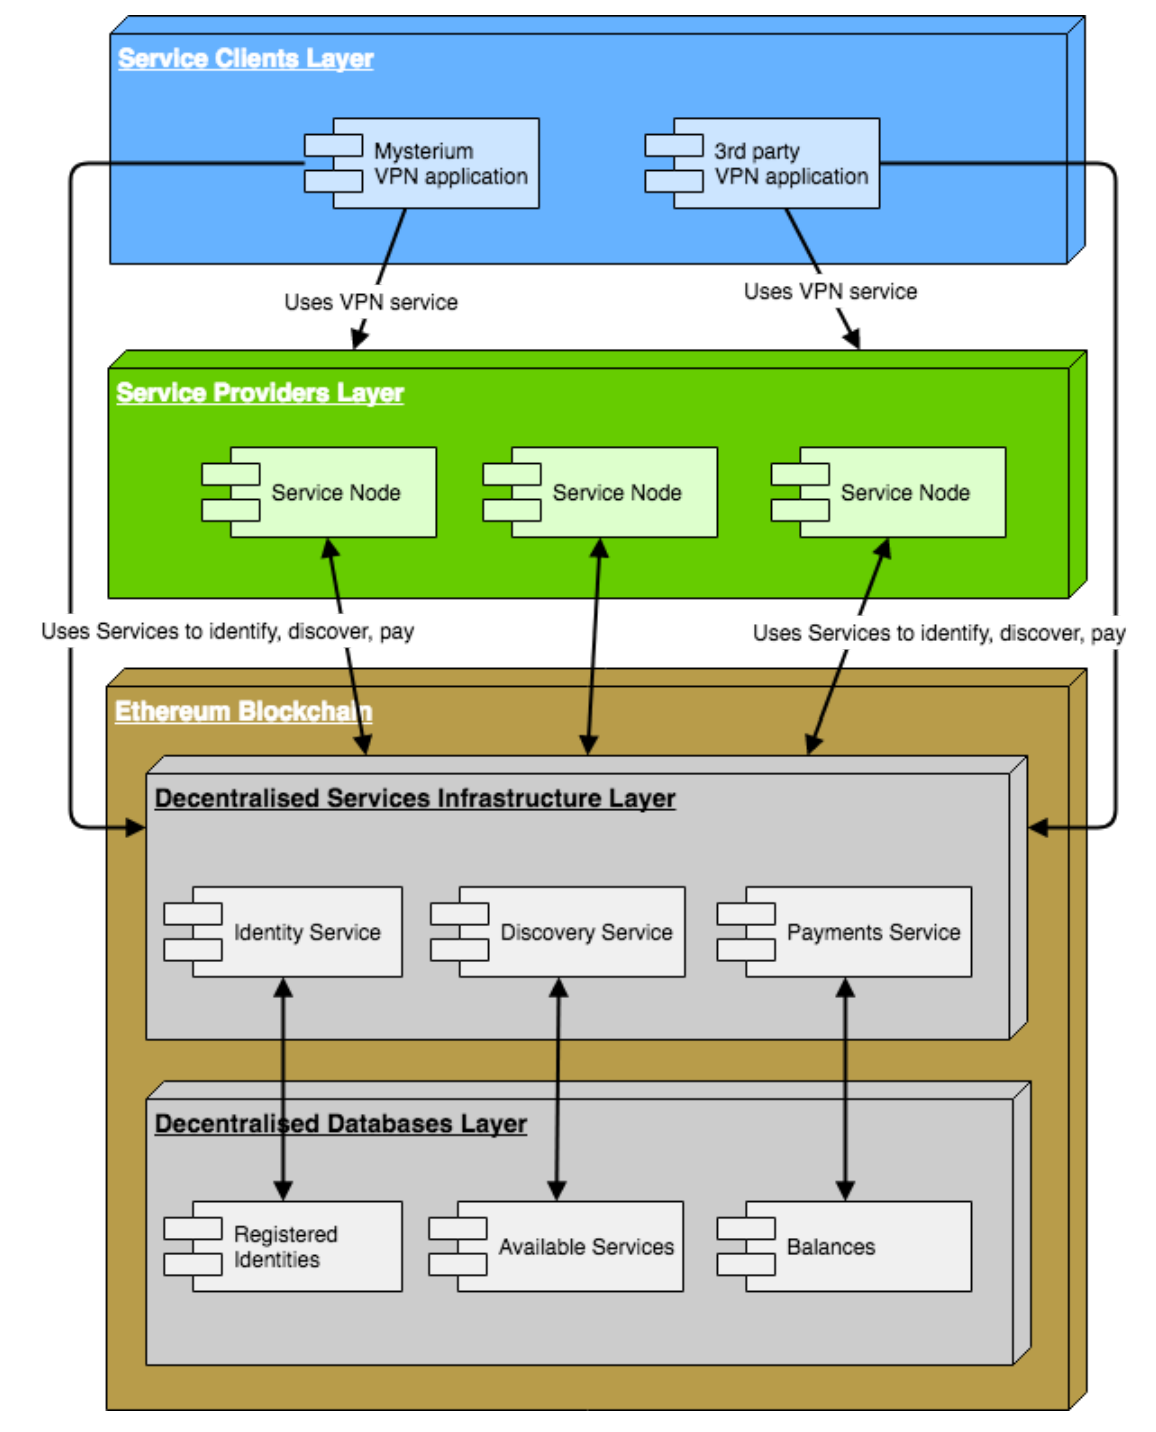
\includegraphics[width=0.5\linewidth]{images/mysterium_architecture.png}\\
		\small{\textit{The Mysterium Network architecture}}
	\end{center}
	\bigbreak

	As a general workflow description, Mysterium starts by collecting all the agents' service proposals and presents them to the clients. Then it registers the client's intention to pay for the agent's service chosen by the user and creates the VPN connection between the two points. The outcome of each transaction is saved in the blockchain.\\
	
	\bigbreak
	To implement all the functionalities just said, Mysterium has four core components inside its architecture:
	\begin{itemize}
		\item \textbf{Ethereum Blockchain} allows running decentralized code with smart contracts, enabling reliable services and payment handling.
		\item \textbf{Identity service and database of registered identities} ensure the proper identity acknowledgment between client and service provider.
		\item \textbf{Discovery service and database of available services} provide means to announce the availability of VPN services and to pick the most suitable VPN service.
		\item \textbf{Payment service and database of balances} allow secure promise-based micropayments for services.
	\end{itemize}

	\subsubsection{Identity Service}
	The \textbf{identity service} manages the network identities that every node needs. A single node can create one identity or more, and each of them consists of a public and a private key. The last 20 bytes of the hash function, applied on the public key, is the unique ID used to identify the node into the network. To publish a new identity so that other network members can reach it, Mysterium uses the smart contract mechanism. The private and public keys are used to validate the signature for the communication between the nodes.\\
	The blockchain mining process appends the public key and the unique ID to the Ethereum blockchain after the node pays a fee to the network. This amount of money has the purpose of giving value to the identity. In such a way, to abandon the identity and create a new one is unattractive because it is expensive, but not impossible.\\ 
	We will discuss those aspects later, but we can surely say this is the first barrier to block in mass identity creation.\\
	Furthermore, the user benefits in using the same identity because it is possible to rebuild his transaction history and his balance from the Ethereum blockchain, making the user more predictable and thus trustworthy for service providers.\\

	\bigbreak
	\begin{center}
		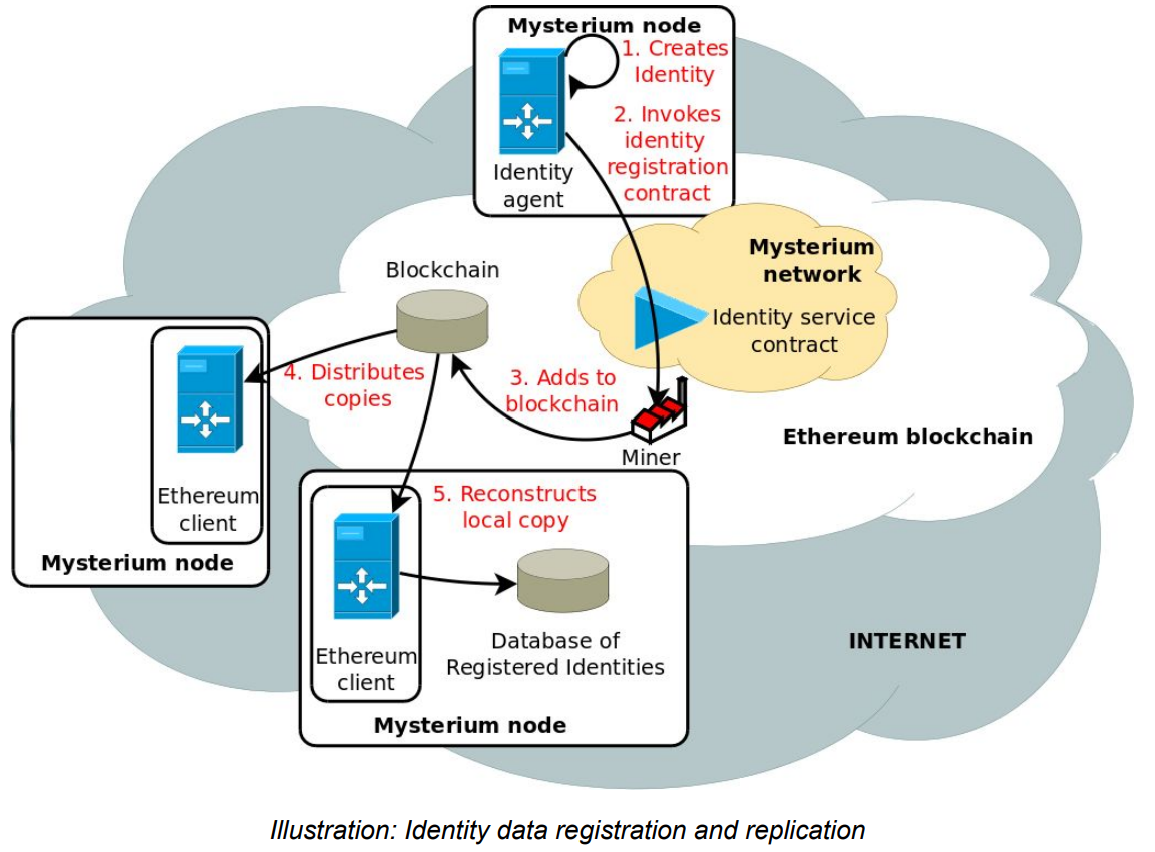
\includegraphics[width=1\linewidth]{images/mysterium_identity_creation.png}\\
		\small{\textit{Identity data registration and replication}}
	\end{center}

	\subsubsection{Service Discovery}
	The \textbf{service discovery} provides the list of service proposals available in the network. The service posts its service offer characterized by some service parameters: those parameters can be the VPN application the provider supports, the provider's connection IP address and port, the provider's server location, or the bandwidth per session. Then, the miners append the proposal to the blockchain, making it publicly available for everyone.\\

	\bigbreak
	\begin{center}
		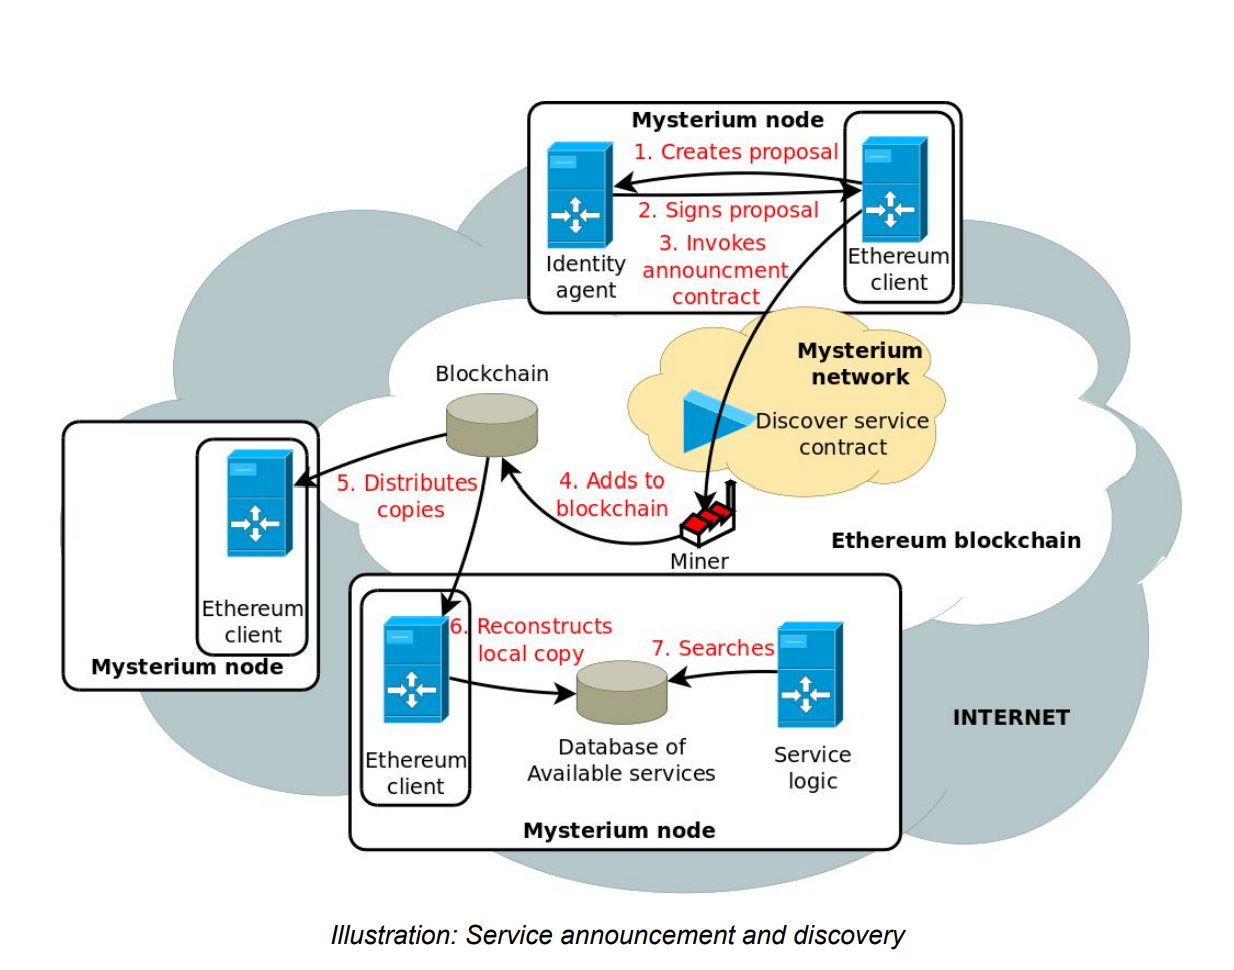
\includegraphics[width=1\linewidth]{images/mysterium_service_announcement.png}\\
		\small{\textit{Service announcement and discovery}}
	\end{center}
	
	\subsubsection{Payments Handling}
	Ethereum blockchain holds all the mechanisms for the \textbf{payments handling}. Therefore everyone needs an account to operate in the Mysterium Network. To advance a request, the consumer has to deposit currency in his wallet. Then, he can ask for a connection to a provider who has previously published a service proposal. Mysterium describes this step as a promise creation because the client effectively promises he will pay when the service ends. Positively clearing a promise is the everybody's best interest, the producer and the consumer, since a canceled promise marks the consumer's history hitting his reputation for future connections.\\
	From what we have described so far, it seems the consumer can decide to avoid paying for the used service: technically, it is possible, but realistically there are some considerations to be made.\\
	First of all, as previously described, identity creation takes money to be completed, and for any new connection, the user's balance has to be positive. In any case, the blockchain records any connection result so that everybody can rebuild the user's history at any moment. Therefore, it is possible to deduct the user's reputation based on its history.\\
	Using this reputation, the provider can decide to block his service to all users that have a low reputation caused by an unpaid precedent. On the other hand, other providers allow new users' connections with a low reputation but at a high price, accepting the risk of having an unpaid transaction.\\
	
	\subsection{Components}
	The core application is called \textbf{node}. It's written in GoLang, a new program language made by Google that is having a high adoption in the last years. The node creates a local webserver to connect to the network, manages the cryptocurrency wallet, and initiates the VPN connection as a client or manages the incoming connection as a server. Mysterium leans on famous VPN applications, which are OpenVPN and Wireguard.\\
	The node can be run in two modes, as a client or as a server, and it is managed via command-line interface or RESTful API, called TequilaAPI, exposed in the localhost.\\
	\bigbreak
	The main functionalities of TequilaAPI concern:
	\begin{itemize}
		\item the authentication,
		\item the connection,
		\item the identities,
		\item the location,
		\item the proposals,
		\item the service operations in provider mode
		\item other minor features
	\end{itemize}
	\bigbreak

	TequilaAPI is used by the client's application to manage the connection and for diagnostic operations.\\
	Mysterium developed a desktop client written using Electron, which uses the TequilaAPIs. The node is also available as a ready-to-use Docker image and published on the Docker Hub.\\
	On the mobile side, Mysterium is present with its multiplatform app that works only as a client.\\
	
	\bigbreak

	\subsubsection{Technical description}
	We have chosen the Linux platform and OpenVPN as the VPN application to describe the technical aspect, but the same conclusion can be reached with different configurations.\\
	When the Mysterium application starts, it calls OpenVPN, which sets up its network environment. OpenVPN creates a virtual network device used to encrypt and decrypt the traffic. These devices reside in the kernel and are entirely virtual, which means there is no hardware on their back.\\
	They can be of two types, TAP or TUN.\\
	The TAP type is used to simulate a link layer device, which means the corresponding ISO model level it refers to is number two. Therefore, a TAP interface handles the transmission of the data frames between two nodes on the same physical layer. The behavior is equal to a bridge device: to connect two separates networks as if they were one.\\
	On the other hand, the TUN type is, in the ISO model, one layer above, working at level three. A TUN interface handles packets, such as Internet Protocol packets. The main functions include port forwarding, host addressing, and traffic control, for example. The behavior is, in this case, equal to a router device: to connect two separates networks allowing their communication but keeping them independent.\\
	Usually, the TUN type is the most used, since the TAP type brings some limitations such as it cannot be used with Android or iOS devices, causes higher overhead on the VPN tunnel, and scales poorly.\\
	The following schema describes an example of a scenario where the network has two ethernet cards, one public and one internal.\\
	As described in the following picture, the virtual TUN interface created by OpenVPN is \lstinline{tun0}, the public interface is \lstinline{eth0}, and the internal interface is \lstinline{eth1}.\\

	\bigbreak
	\begin{center}
		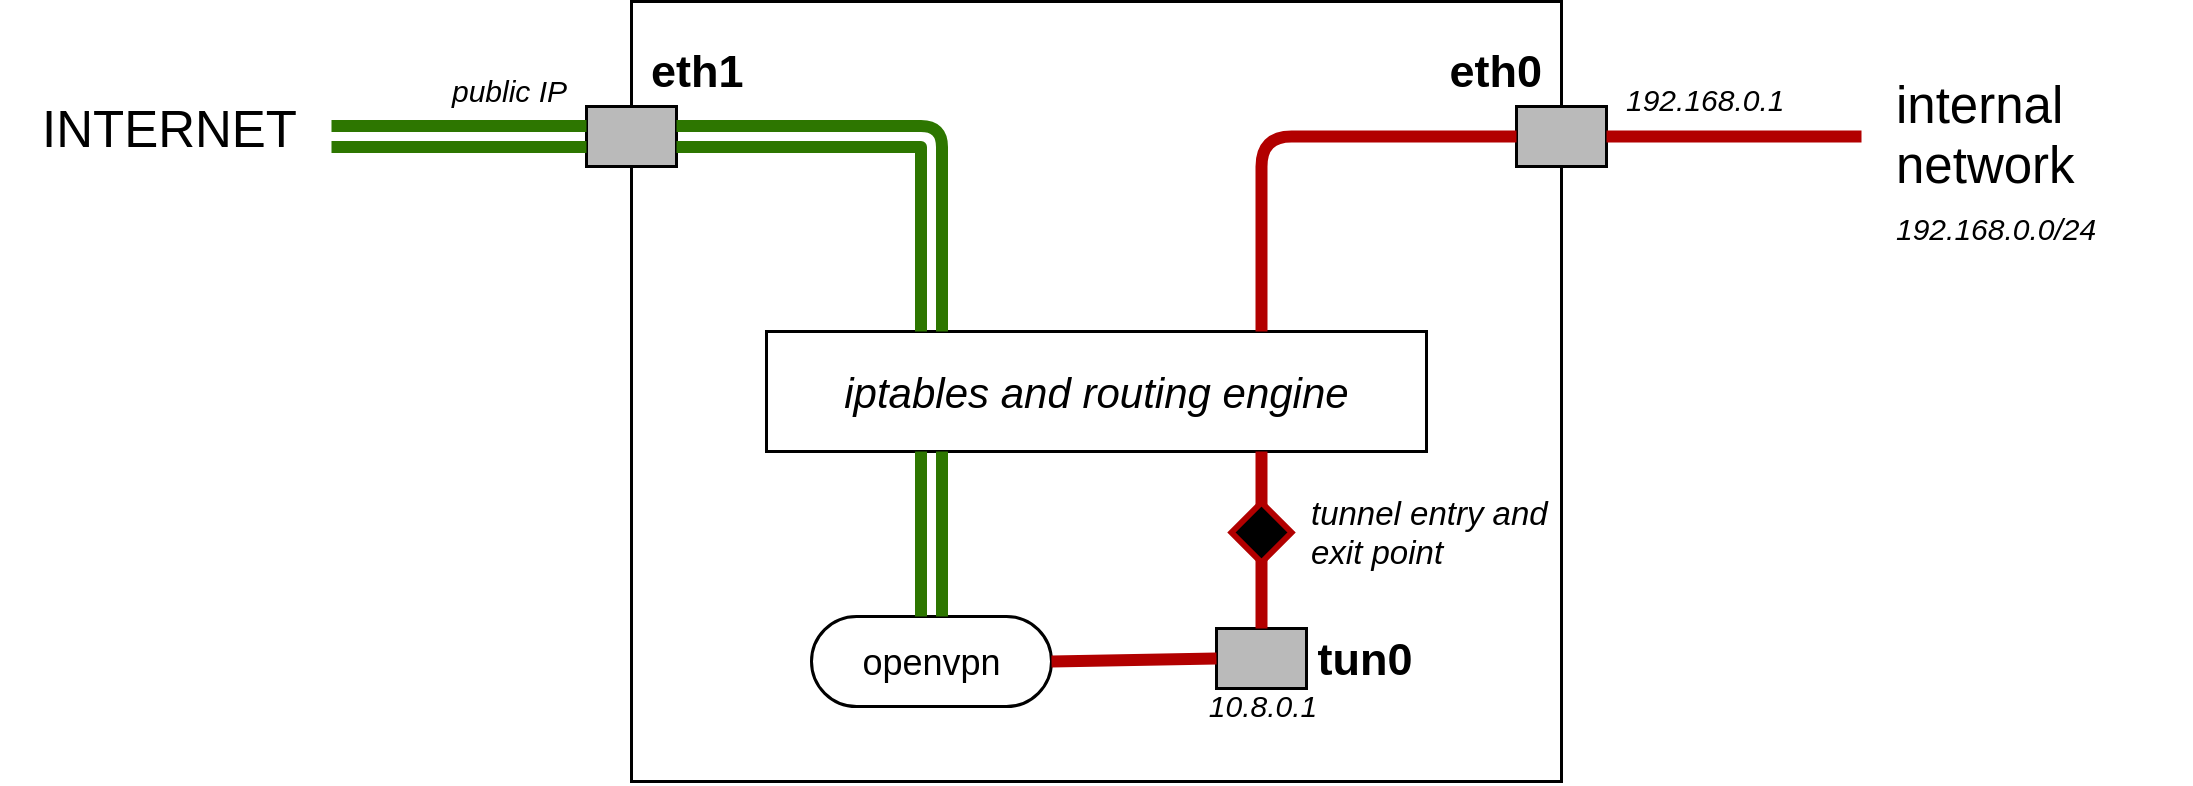
\includegraphics[width=1\textwidth]{images/openvpn_routing_setup.png}\\
		\small{\textit{OpenVPN routing setting}}
	\end{center}
	\bigbreak
	When a packet arrives at the \lstinline{eth1} interface, OpenVPN picks it up, decrypts it, and sends it to the \lstinline{tun0} interface. The \lstinline{iptables} and the routing engine filter and masquerade the packet and send it to \lstinline{eth0}, where it becomes available to the final receiver.\\
	In the other direction, when the packet arrives at \lstinline{eth0} interface, \lstinline{iptables} and the routing engine apply their rules to filter and masquerade, and then they forward it to \lstinline{tun0} interface. Thus, OpenVPN picks it up, encrypts the data, and sends it to the public \lstinline{eth1} interface.\\
	In our scenario, the network configuration is slightly different and does not include an internal interface network. OpenVPN sends the traffic coming from \lstinline{tun0} to the public interface \lstinline{eth0} on a specific port. The client application listens on that port, and the OpenVPN client decrypts the received data.\\
	\bigbreak

	\begin{center}
		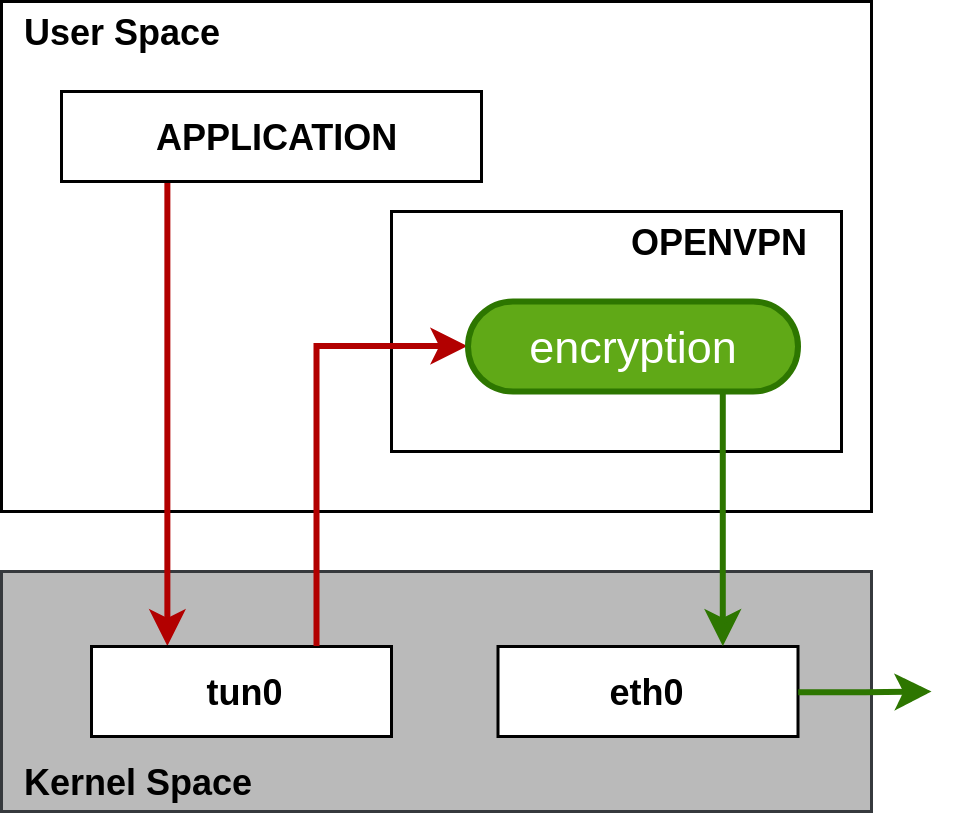
\includegraphics[width=0.5\textwidth]{images/openvpn_tun_interface.png}\\
		\small{\textit{OpenVPN TUN interface}}
	\end{center}

	\subsubsection{Start a node}
	There are two ways to start a Mysterium node. The first one is using the Docker image: Docker is a platform that uses the OS virtualization to deliver software in packages called containers. The image contains all the specifics that the application requires to be executed.\\
	From the software image, Docker creates as many containers as we instantiate, and they are the virtualized software we will use.  We can think of the software image as the house project and the software container as the real house construction. As the house construction can have personalizations, either the container is set up passing parameters to customize the network, the storage, or other settings such as the resources allocated by Docker to the single container.\\
	\bigbreak
	With the following command, we pull the image of the Mysterium node from the Docker platform:\\
	\bigbreak
	\begin{lstlisting}[frame=single]
		docker pull mysteriumnetwork/myst
	\end{lstlisting}
	
	Then, we create the container using:\\

	\begin{lstlisting}[frame=single]
		sudo docker run --cap-add NET_ADMIN --net host --name myst -d mysteriumnetwork/myst service --agreed-terms-and-conditions --openvpn.port 1194
	\end{lstlisting}

	The parameters specify, from left to right:
	\begin{enumerate}
		\item to add the network capability to the operative system, which is Linux,
		\item to connect the container to the net,
		\item to name the container \lstinline{myst},
		\item to run the container in background mode and detach it from the shell.
	\end{enumerate}

	The remaining values are passed to the Mysterium software. The \lstinline{service} value means Mysterium node starts as a node, thus a service provider, instead of a client, the next one is to agree on the terms and conditions, and the last one is to set up the OpenVPN port.\\
	When the container is up and running, we can check the logs using:

	\begin{lstlisting}[frame=single]
		sudo docker logs -f myst
	\end{lstlisting}
	
	We can find relevant details reading the log, such as the identity registration and the node proposal:
	\begin{lstlisting}[frame=single]
		...
		[Mysterium.api] Identity registered: 0x4cd126119cd14e38c90e34dd8b6e0e2174b71123
		[Mysterium.api] Proposal pinged for node: 0x4cd126119cd14e38c90e34dd8b6e0e2174b71123
		...
	\end{lstlisting}

	The identity registration is the unique ID assigned from the network to the node. With this ID, it is possible to discover it, its connection details, and transaction history on the Mysterium Network website.\\
	
	
	The second way to install the Mysterium node is using the Debian package. To manage its execution, we use the \lstinline{systemctl}, a management tool for controlling the init system:\\
	We run 

	\begin{lstlisting}[frame=single]
		sudo systemctl daemon-reload
	\end{lstlisting}

	to reload the daemon after the changes to the node settings, and 
	
	\begin{lstlisting}[frame=single]
		sudo systemctl restart mysterium-node
	\end{lstlisting}
	
	to reload the node.\\

	If the node is up and running, it exposes a web interface on the localhost available at port 4449, where it is possible to control the service status and see connection statistics.
	
	\subsubsection{Connect to a node}

	When the node works, the simplest way is to use the mobile or desktop client applications that provide a graphical interface to choose the server node and establish the connection. In a few seconds, the Mysterium network creates the connection record in the blockchain, initializes the connection and, then, the VPN takes place.\\

	Another way to connect to the service provider is using the command-line interface the node as a client exposes. Referring to the node installed by the Debian package, the command to run the node and control it is:\\
	
	\begin{lstlisting}[frame=single]
		myst cli
	\end{lstlisting}

	We then enter in a view where we can perform the operations on the node that regard the identity management, the connection creation, and the status diagnostic.

	\subsubsection{Iptables}

	The \lstinline{iptables} is a framework to manage the network decisions. It is based on the Netfilter kernel component, which exposes a set of hooks that are triggered at specific points of the network stack. Every packet that enters the networking system will trigger these hooks as it proceeds through the stack so all the programs that register with these hooks can interact with the traffic.\\
	\bigbreak
	Five different hooks correspond to different points of the stack:\\

	\bigbreak
	\begin{itemize}
		\item \lstinline{NF_IP_PRE_ROUTING}
		\item \lstinline{NF_IP_LOCAL_IN}
		\item \lstinline{NF_IP_FORWARD}
		\item \lstinline{NF_IP_LOCAL_OUT}
		\item \lstinline{NF_IP_POST_ROUTING}
	\end{itemize}
	\bigbreak

	\bigbreak
	\begin{center}
		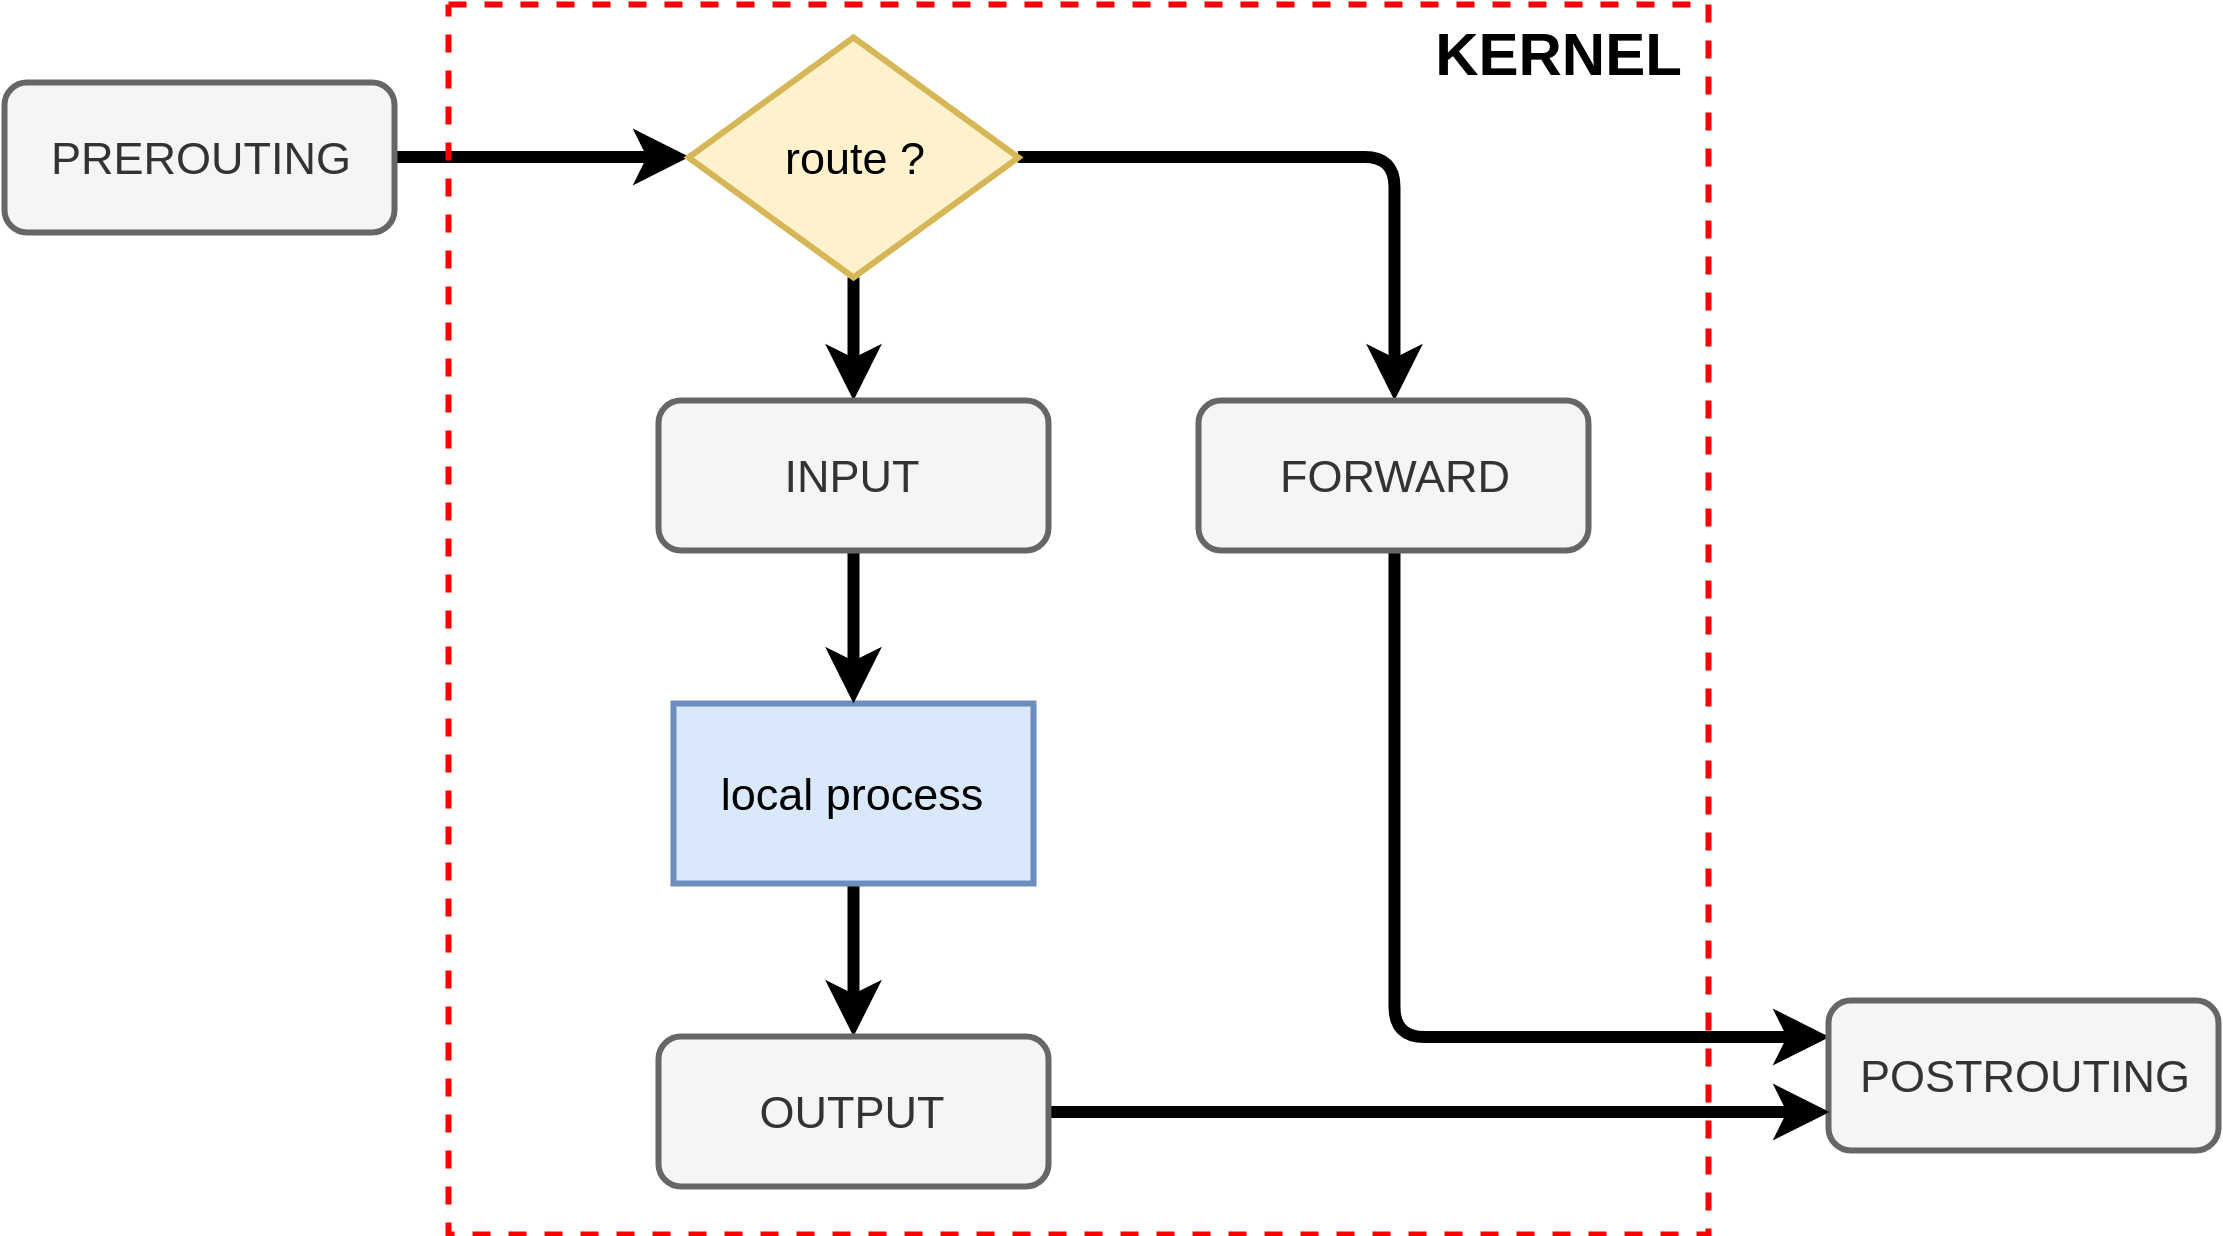
\includegraphics[width=\linewidth]{images/iptables_hooks.png}\\
		\small{\textit{Hooks in the internal network stack}}
	\end{center}
	\bigbreak
	Iptables is mainly used as a firewall which organizes its rule in tables and chains. The tables classify the rules according to the type of decision that regards the packet.\\
	The available tables are the filter table, the NAT table, the Mangle table, the Raw table, and the Security table.\\
	The chains correspond to the available hooks, therefore iptbales has the \textbf{prerouting}, \textbf{input}, \textbf{forward}, \textbf{output}, and \textbf{postrouting} chains.\\
	The following table explains the triggering logic and execution precedence.\\
	\bigbreak
	
	\begin{center}	
		\begin{tabular}{|l|c|c|c|c|c|}
		\hline
		\textbf{\begin{tabular}[c]{@{}l@{}}Chains\\ Tables\end{tabular}} & \rotatebox[origin=c]{90}{\textbf{PREROUTING}}    & \rotatebox[origin=c]{90}{\textbf{INPUT}}         & \rotatebox[origin=c]{90}{\textbf{FORWARD}}       & \rotatebox[origin=c]{90}{\textbf{OUTPUT}}        & \rotatebox[origin=c]{90}{\textbf{POSTROUTING}}   \\\hline
		\textit{ruoting decision} & & & & X & \\\hline
		\textbf{raw} & X & & & X & \\ \hline
		\textit{connection tracking enabled} & X & & & X & \\\hline
		\textbf{mangle} & X & X & X & X & X \\\hline
		\textbf{DNAT (NAT)} & X & & & X & \\ \hline
		\textit{routing decision} & X & & & X & \\ \hline
		\textbf{filter} & & X & X & X & \\ \hline
		\textbf{security} & & X & X & X & \\ \hline
		\textbf{SNAT (NAT)} & & X & & & X\\	\hline
		\end{tabular}
		\bigbreak
		\small{\textit{Hooks and triggers}}
	\end{center}

	
	\bigbreak

	The packet triggers the hooks from the first row going down to the bottom of the table. It enters the chain depending on the routing decisions that are made based on its direction, incoming or outgoing, and whether the filtering rule accepts the packet.\\
	\bigbreak
	The chain traversal order is the following:\\	
	\textbf{Incoming packets destined for the local system:}\\
	$\hbox{PREROUTING} \rightarrow \hbox{INPUT}$\\
	\medskip
	\textbf{Incoming packets destined to another host:}\\
	$\hbox{PREROUTING} \rightarrow \hbox{FORWARD} \rightarrow \hbox{POSTROUTING}$\\
	\medskip
	\textbf{Locally generated packets:}\\
	$\hbox{OUTPUT} \rightarrow \hbox{POSTROUTING}$\\

	\bigbreak
	Every chain is a list of rules. Every packet is checked against each rule and, if the matching component checks, iptables executes an action.\\
	The rule can match the packet depending on the protocol type, the source or destination address, or packet, among other criteria.\\
	The action called target, which is triggered if the rule matches, can be of terminating or non-terminating type.\\
	The terminating type target causes the packet to exit the chain after a verdict that can be to allow or to drop the packet. The non-terminating type target causes the packet to continue its evaluation in the chain. There can be any number of non-terminating targets before a terminating one.\\
	A very used non-terminating target is the jump action: a rule can decide to jump a packet into another chain, and when that chain finishes the rules check, the execution comes back to the previous chain. This way is useful to organize the rules in chains based on their purposes.\\
	
	\bigbreak
	\begin{center}
		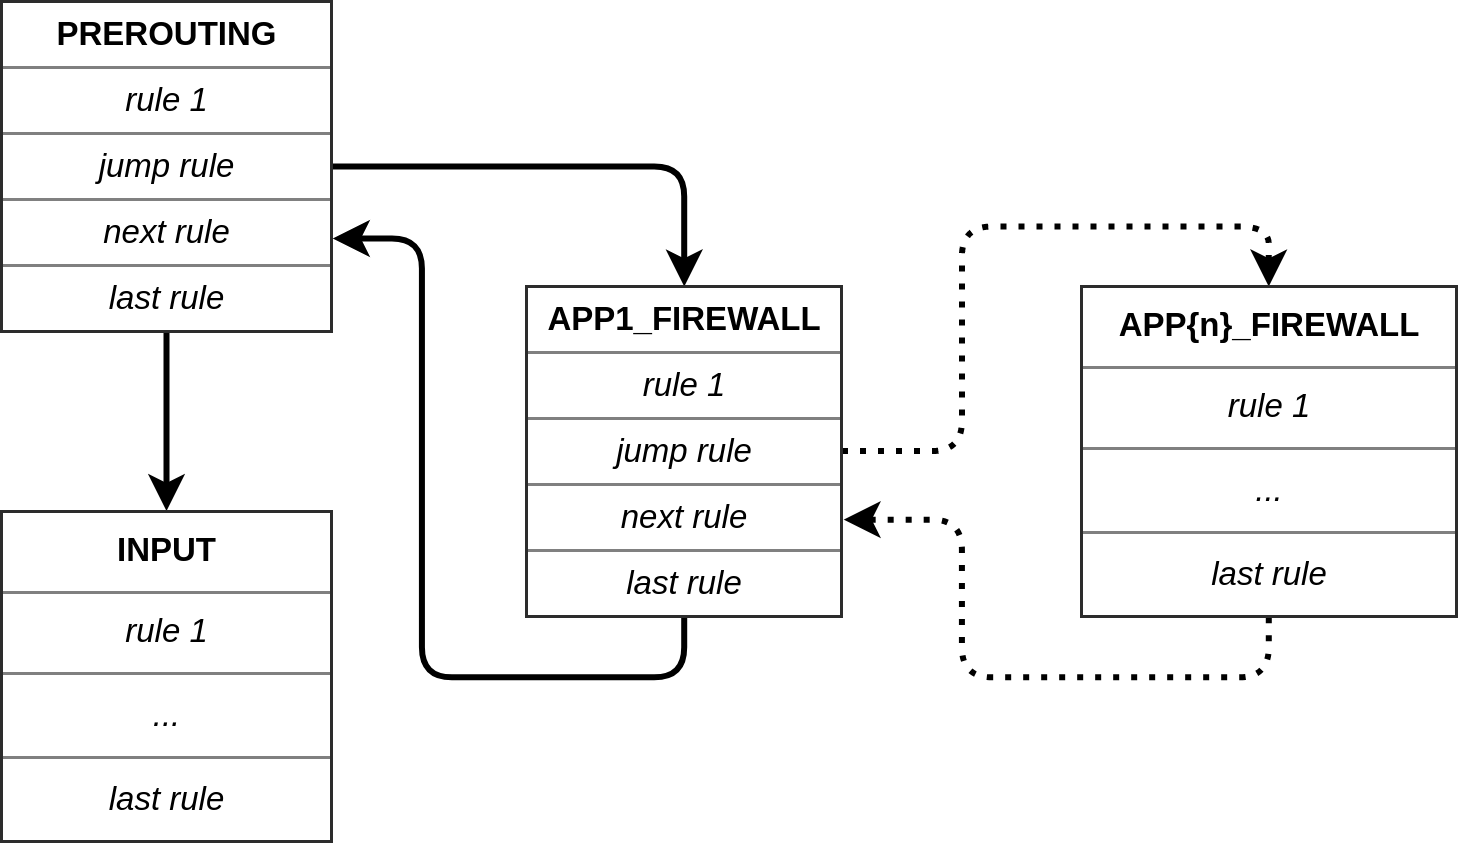
\includegraphics[width=\linewidth]{images/iptables_jump_chains.png}\\
		\small{\textit{The \lstinline{iptables} jump rule}}
	\end{center}
	\bigbreak

	With \lstinline{iptables}, it is possible to build firewalls and control systems to manage the computer network efficiently.


	\subsection{Design vulnerabilities}

	Mysterium is a complex system that integrates components of different types. The distinct nature of these components and their conjunction opens to new vulnerabilities scenarios where the focus is on the system overall and how the elements dialog each other.\\
	In the following chapter, we provide considerations on the Mysterium Network system concerning its components and their integration. To do this, we assumed some components behaviors and their impact on the system because Mysterium does not implement them yet, at this time. Indeed, Mysterium project is under development, which plans to have a fully decentralized network in 2021.\\
	\bigbreak

	We classify the several aspects that, on a project like Mysterium, must be considered to evaluate its design vulnerabilities based on:
	\begin{itemize}
		\item the position in the network: starting, middle or endpoint point;
		\item the step of the flow: the service proposals, the promise issuing, the transaction closing, and other steps;
		\item the operations on the passing data: sniffing, filtering or crafting the data;
		\item side channels attack and other particular scenarios.
	\end{itemize}
	
	\subsubsection{The position in the network}

	In the simplest configuration, the network includes a starting point that is the service consumer node and an endpoint, which is the service provider node. The VPN tunnel connects the two nodes and encrypts their traffic. The service node, as previously described, is the consumer's exit point to the internet.\\
	We consider secure the traffic passing through the VPN tunnel because it is encrypted, not secure otherwise, that is from the provider to the internet.\\

	\bigbreak
	\begin{center}
		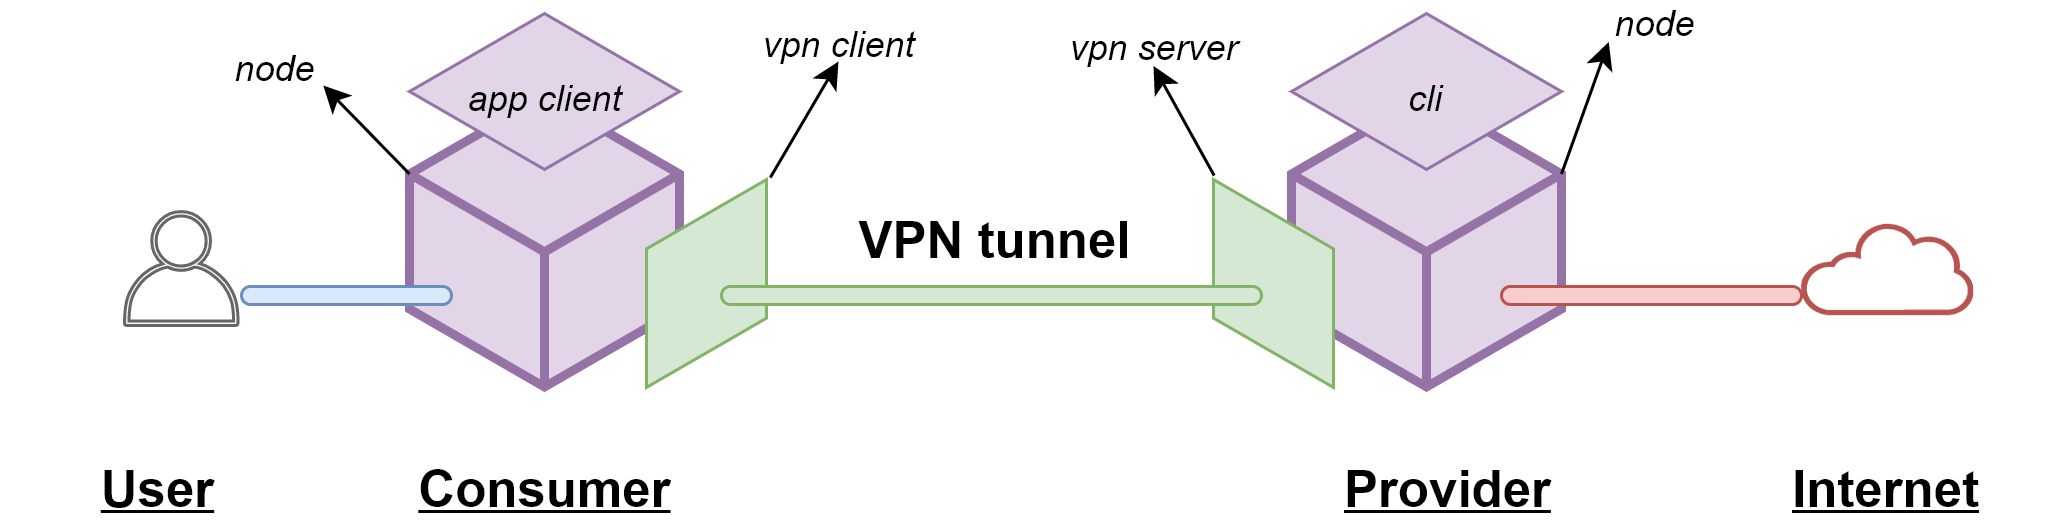
\includegraphics[width=1\linewidth]{images/client_server_vpn_connection2.png}\\
		\small{\textit{The VPN connection between a consumer and a provider}}
	\end{center}
	\bigbreak

	The exit nodes connect two areas with two different security levels: for this reason, it is sensitive by default and without specific precautions can be the weak link of the system.\\
	The Tor network has a similar problem. Tor stands for The Onion Router, and it is a network of peers where the user's encrypted traffic is sent into, and it bounces multiple times before getting an exit node from where, finally, it reaches the external resource.\\
	The traffic is encrypted for each bouncing, except the last one, where it must be in clear to connect to the internet resource. The end node's role is to decouple the encrypted network from clear internet, and this makes it so valuable. If an exit node is malicious, it can potentially understand all the data passing through it and going to the internet resource.\\
	\bigbreak
	Dan Egerstad is a Swedish computer security consultant. He intercepted thousands of diplomatic emails setting up malicious exit nodes around the world and sniffing the connection between them and the clear internet \cite{exitnodeTOR}.\\
	To discover malicious nodes in the Tor network, another Swedish researcher built up a website with a login and a system to count the login attempts. Then, he used multiple Tor paths with different exit nodes to access the page. The system counted more login attempts that the researcher have done: this means some exit nodes sniffed the connections, caught the username and password, and tried to login by themselves \cite{exitnodeTOR2}.\\
	In both cases, the use of HTTP instead of HTTPS, or of other unencrypted protocols, has been necessary, but the research aim was to demonstrate the exit nodes' critical role: there still are many protocols and applications that do not use encryption for their traffic.\\
	The conclusion is that Tor's end nodes are the weak link of the system when the users use it as an end-to-end encryption network, rather than an anonymization network, as well as Mysterium Network end nodes.\\
	For this reason, many of the conceptual vulnerabilities held by the exit node of Tor can be applied to a Mysterium Network exit node. But we want to point out a difference between Tor and Mysterium networks: the type of target users of the two projects.\\
	The Tor's users use it to accomplish specific online activities where the identity obfuscation is mandatory. For the rest of the actions, Tor is not efficient, can be blocked by ISP and, in some countries, is even banned.\\
	The Mysterium Network users, instead, use it for a broader range of online activities, and we can assume a persistent connection to the VPN network with almost no impact on the user's system. In this direction, the implementation of the mobile app is crucial: smartphones are becoming the first device from where people access the internet. The capability to have a device connected all the time with the VPN network provides a desirable security level for consumer uses.\\
	This scenario, however, introduces more vulnerabilities simply because the network is used for more activities, and many protocols and applications still use unencrypted communication.\\
	In conclusion, the provider manages all the traffic from the VPN tunnel, both incoming and outgoing, and because it has not the VPN encryption, he can potentially perform all the manipulation he wants. We will discuss further this scenario analyzing the technical solutions and providing a practical example to exploit in Craftberry chapter.\\
	\bigbreak
	An improved configuration implies one or more middle points between the consumer and the provider. Those points are called hops, and they act similarly to the provider node since they forward the traffic.\\
	Mysterium did not implement those hops in the network yet. Therefore we make a hypothesis on its possible implementation.\\
	As well as for the provider nodes, we can suppose there is a distributed list of the forwarder nodes. When the consumer chooses the provider, and they agree to issue a payment promise, the network picks a node from that list to place it as the hop. The middle node receives a new VPN connection from the consumer and creates a new VPN connection to the provider. He technically builds and manages two different VPN tunnels: it takes encrypted data from one side, decrypts them, and encrypts again to send on the other one.\\
	The scenario is similar to the end node because the middle node holds unencrypted data in the forwarding action.\\
	The following picture well describes the situation with even more than one hop. We would have a segmented connection, called multihop connection, between the ends, where all the hops can perform unwanted operations on the traffic.\\
	
	\bigbreak
	\begin{center}
		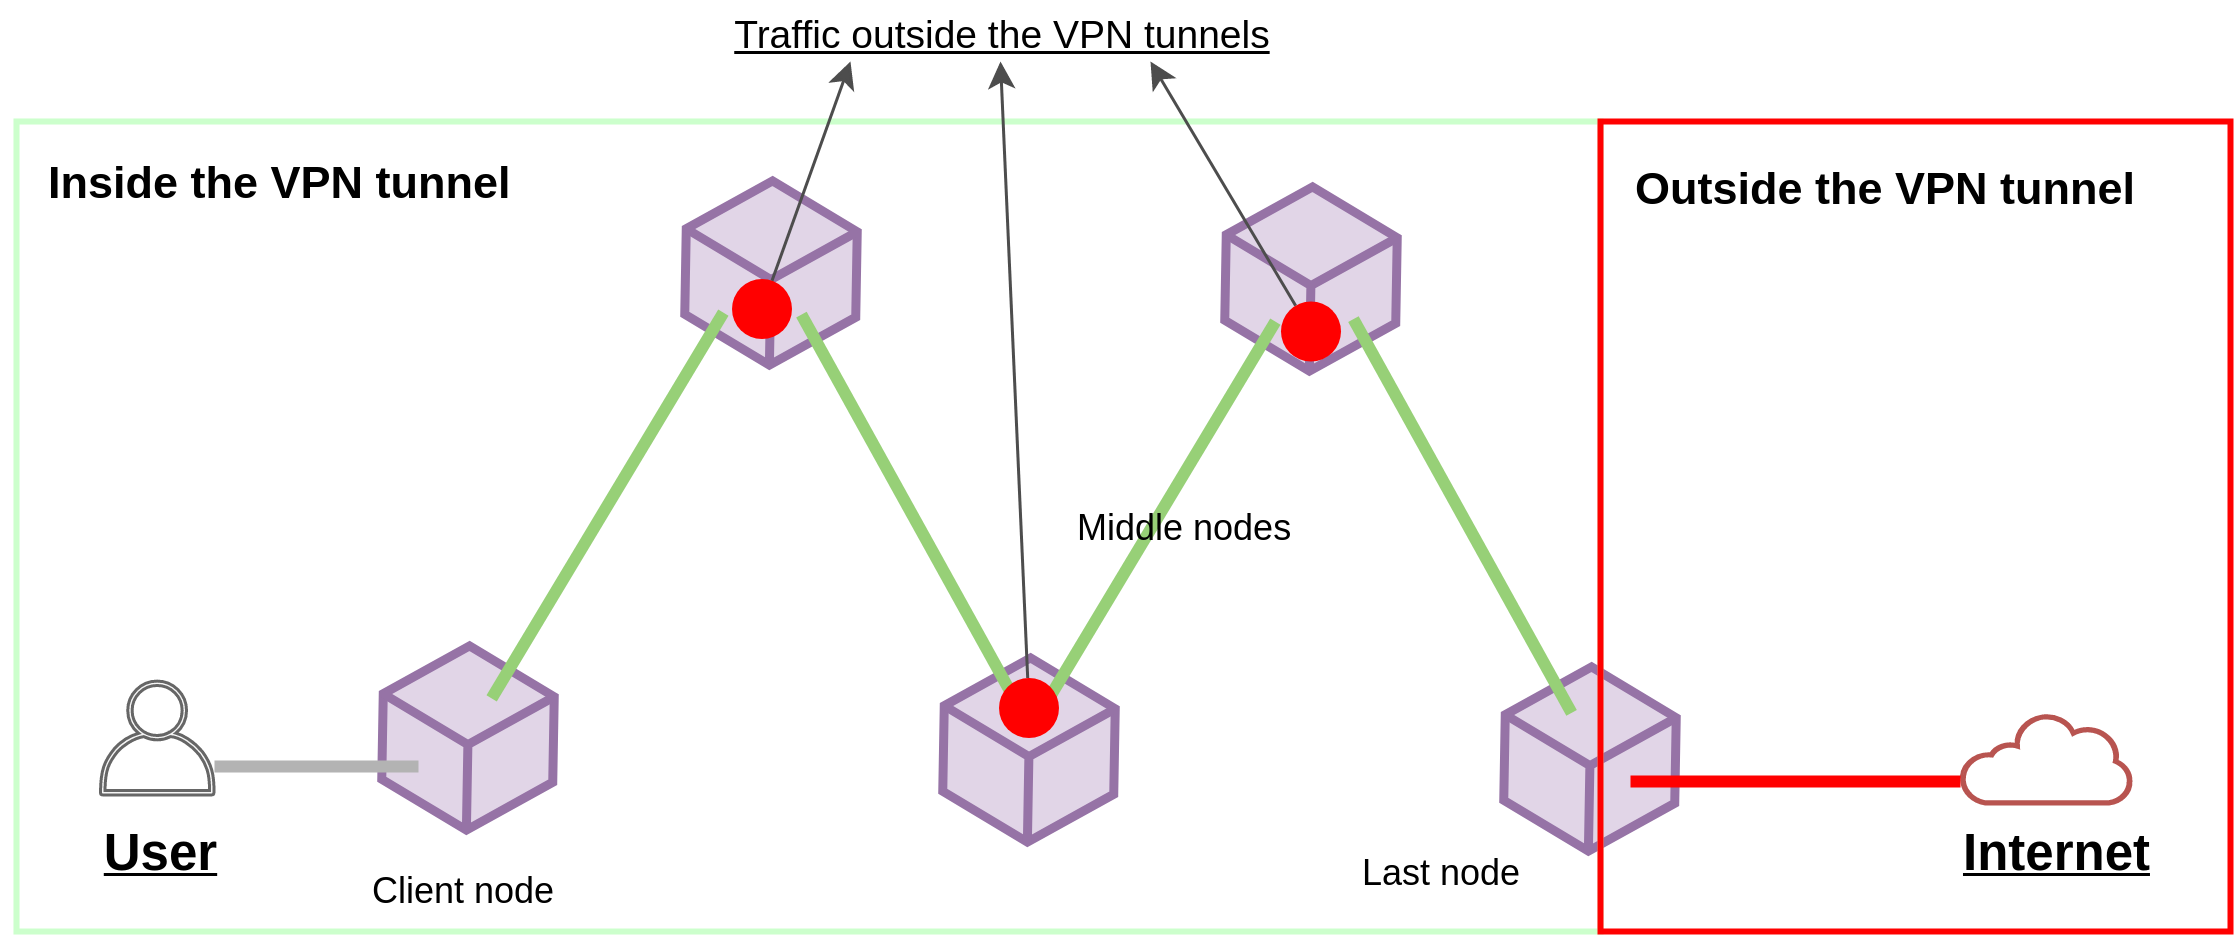
\includegraphics[width=1\linewidth]{images/client_server_vpn_multihop_connection.png}\\
		\small{\textit{A multihop connection a consumer and a provider}}
	\end{center}
	\bigbreak

	Mandatory would be an additional encryption layer end to end, over the VPN encryption between each node, that the consumer and provider have to manage. This second encryption solves the multihop data exposing because the middle nodes would manage only data encrypted by the second layer. The cons are that it increases the computational load.\\

	\bigbreak
	\begin{center}
		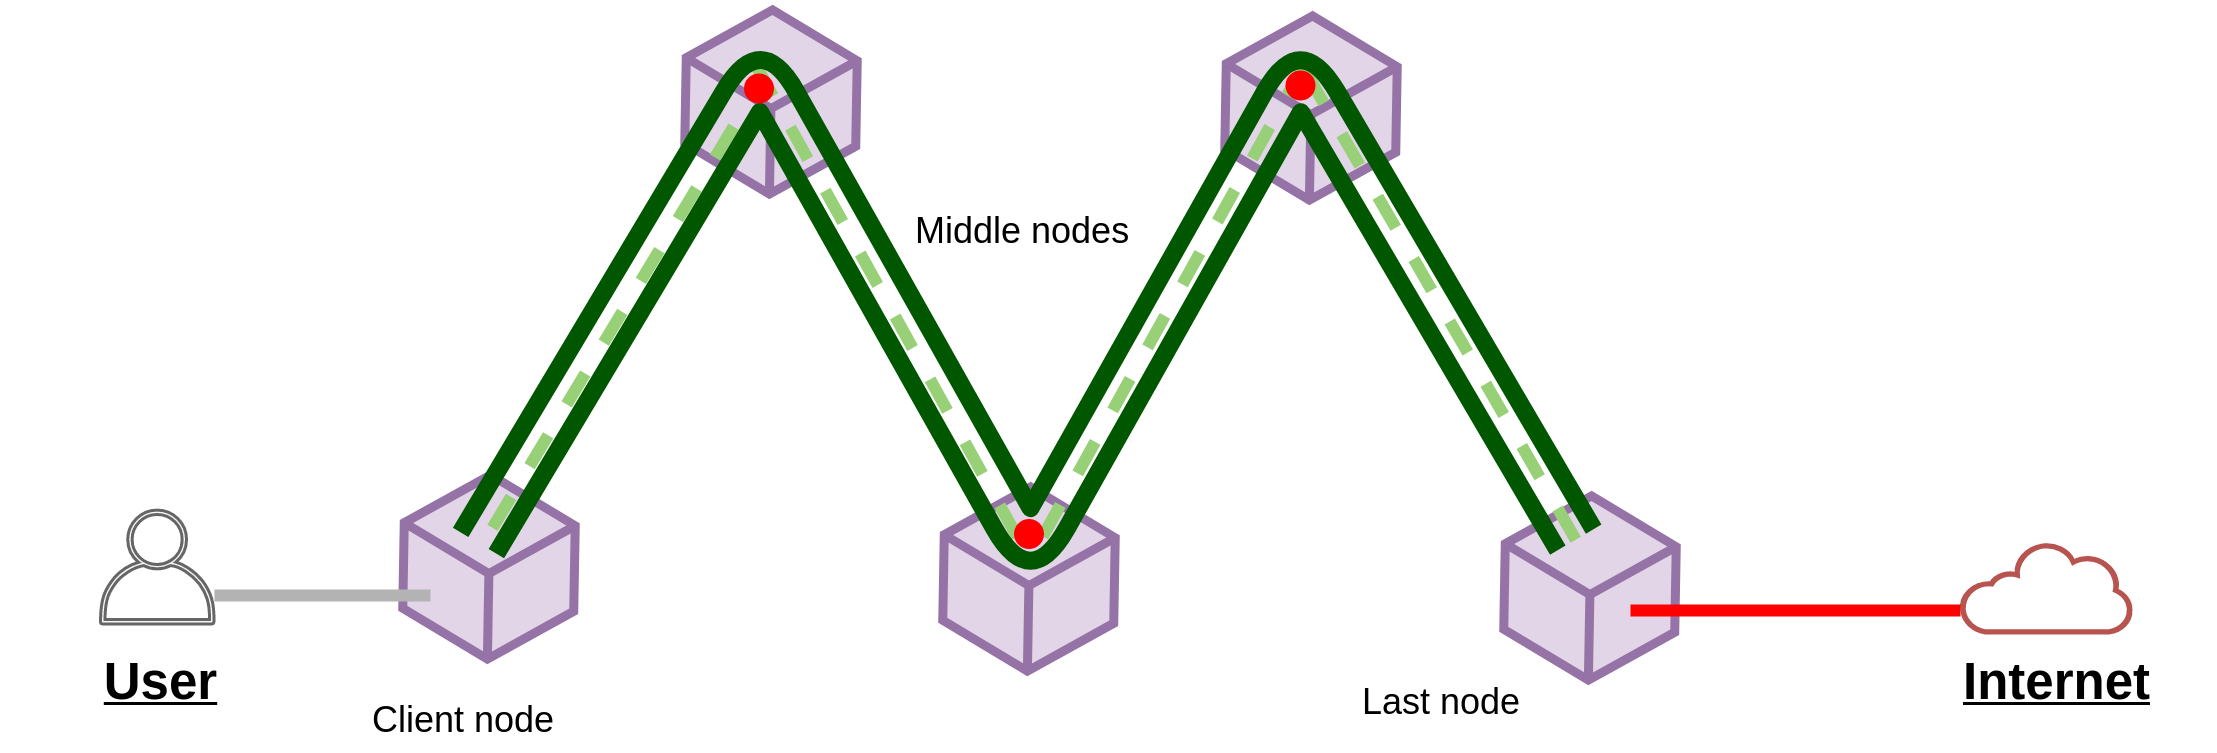
\includegraphics[width=1\linewidth]{images/client_server_vpn_multihop_connection_e2e_enc.png}\\
		\small{\textit{A multihop end-to-end encrypted connection}}
	\end{center}
	\bigbreak	

	The vulnerabilities, in this scenario, are restricted to all the operations that concern the traffic shape, with no abilities to understand it. These actions hit the quality of service, a class of attacks that aim to lower or even block the service.\\
	Many traffic shapes operations can be performed on a connection: the simplest and the fastest is on the traffic speed, and it does not need to understand the content at all.\\
	\bigbreak
	A demonstration of how a middle node can slow down the data speed that it forwards, is given using a Linux package called \lstinline{tc} \cite{tc}. It stands for Traffic Control, and it is created and used for service quality analysis.\\
	With the following command, we instruct the network manager to apply a delay of 500 milliseconds for every packet sent to the interface \lstinline{eth0}.\\
	
	\begin{lstlisting}[frame=single]
		sudo tc qdisc add dev eth0 root netem delay 500ms
	\end{lstlisting}
	
	Here is what each option means:
	\begin{itemize}
		\item \lstinline{qdisc}: modify the scheduler (also known as queuing discipline)
		\item \lstinline{add}: add a new rule
		\item \lstinline{dev eth0}: rules will be applied on device\lstinline{eth0}
		\item \lstinline{root}: modify the outbound traffic scheduler (as known as the egress qdisc)
		\item \lstinline{netem}: use the network emulator to emulate a WAN property
		\item \lstinline{delay}: the network property that is modified
		\item \lstinline{500ms}: introduce delay of 500 ms
	\end{itemize}

	With the following command, we delete the delay rule.\\

	\begin{lstlisting}[frame=single]
		sudo tc qdisc del dev eth0 root netem
	\end{lstlisting}

	In this simple way, the traffic speed between the consumer and the provider has a poor quality because one or more middle points are performing this slowing down the operation. From the consumer side, the poor connection is a quality agreement breach, and it affects the service provider's reputation. Since the provider can detect the slow speed, he can suppose the issue is given by the packet path and can propose to the network to change one or more middle nodes. 

	\subsubsection{The flow steps}
	The first and easiest idea to implement to use the system maliciously has already been presented in the introduction: the attacker is the consumer, he creates an account in the Mysterium Network having a positive balance to the cryptocurrency wallet, and then he looks for a service proposal. They agree on the service cost and issue a payment promise. If the consumer does not respect the promise, the result will be registered in the blockchain. In the same way, if the producer alters the service agreement. Therefore, the blockchain is the reputation book of the network, where every user, consumers or providers, can check the other users' reputation. The reputation implementation in this kind of network is an open point.
	
	\subsubsection{Operations on the passing data}

	In this section we analyze the different operation an end node can perform, based on the fact it manages traffic outside the VPN tunnel.\\
	The traffic outside the tunnel is not encrypted by the VPN, but this does not necessarily mean it is not encrypted by itself. Some protocols encrypt data by design. Others do not encrypt or have different structure levels where the lowest have no encryption at all and can be modified.\\ Based on this consideration, the operations that a node can potentially do on the passing data can be grouped in sniffing, filtering, and crafting.\\
	The first step to manipulate the data is to catch it, and we want to show an example of how-to-do. After starting a Mysterium Node on our test server and then establish the connection to it using a Mysterium client, we use \lstinline{tcpdump} to dump the traffic of the network. For the example purpose, we get an online resource hosted on a different server and available using the HTTP protocol, so that the dumped traffic is in clear.\\
	Our example provides an HTTP request to the host www.jafed.xyz with the method GET to obtain a file named test.txt with the content the string \lstinline{cool, you got me sir!}.\\
	The request is executed using curl, a command-line tool for transferring data using various protocols.\\

	\begin{lstlisting}[frame=single]
		curl www.jafed.xyz/test.txt
	\end{lstlisting}
	
	With the following command, instead, we capture the request specifying the output format defined by \lstinline{-v} \lstinline{-n} \lstinline{-l}, then we pipe it to the \lstinline{egrep} command to parse the string and return an easy-to-read text:\\
	
	\begin{lstlisting}[frame=single]
		sudo tcpdump -v -n -l | egrep -i "POST /|GET /|Host:"
	\end{lstlisting}

	A slice of output is\\
	
	\begin{lstlisting}[frame=single]
		GET /test.txt HTTP/1.1
        Host: www.jafed.xyz
	\end{lstlisting}

	that shows we caught the HTTP request.
	
	We use Wireshark to analyze the content, a powerful graphical application for network usages. It supports the \lstinline{pcapng} file extension that \lstinline{tcpdump} uses to save the data.\\
	We print the captured result filtered of the packets of our interest:\\
	
	\begin{lstlisting}[frame=single]
		GET /test.txt HTTP/1.1
		Host: www.jafed.xyz
		User-Agent: curl/7.58.0
		Accept: */*

		HTTP/1.1 200 OK
		Date: Sun, 09 Feb 2020 16:59:45 GMT
		Server: Apache
		Upgrade: h2,h2c
		Connection: Upgrade
		Last-Modified: Thu, 06 Feb 2020 21:49:33 GMT
		ETag: "1ae1c77-15-59def3f9b28fd"
		Accept-Ranges: bytes
		Content-Length: 21
		Content-Type: text/plain

		cool, you got me sir!
	\end{lstlisting}

	We demonstrated we could completely capture the traffic as the exit node of the network. 

	\subsubsection{Side channels attack and particular scenarios}
	In this section, we discuss the possible scenarios that do not directly regard attacks on specific components, but more on how these harmless operations in Mysterium Network lead to vulnerabilities.\\
	In Mysterium Network, the billing method is per the amount of transferred data or per time. Considering the first method, if the exit node is able to higher the volume of the traffic to the consumer, it means the exit node earns money without providing an equal service. A well-designed attack can perform the traffic shaping hiding the increase of traffic volume with network inefficiency.\\
	In the "TCP/UDP" subsection in the Craftberry tool description, we implemented an attack that uses this technic to make multiple copies of the packets using TCP and UDP protocols without the need to understand the content. A more refined attack would be modifying the packet specifically for the used protocol, forcing a communication error so that the protocol corrects it. In this document, we did not focus on those particular cases which are deeply protocol dependent, but the modification aims to increase the transmitted data because the bill is calculated on that.\\
	\bigbreak

	A considerable number of informatic attacks aim to collect traffic data and then sell them to third party organizations for aggressive advertisement campaigns \cite{VPNsellData}. In this perspective, the capability of an exit node to be able to sniff the web requests, as we demonstrated in the previous subsection, make the network vulnerable to this attack.\\

	\newpage
	\section{Craftberry}

	\subsection{The idea}
	Craftberry is a proof of concept tool to demonstrate how a node can sniff, filter and craft the outgoing traffic from an exit node of the Mysterium Network.\\
	It is an application that runs via the command-line interface. It catches the incoming or outgoing packets in line with the packet flow, and it executes different actions accurately implemented to cover many attack and defense cases.\\
	The software is entirely written in C and C++. It uses the \lstinline{nfqueue} extension to move the packet from the kernel space to the user space, where it is crafted and sent back to the kernel space to continue the network traversal. The application uses the PcapPlusPlus library to parse the packet, build its layers, and modify the content.\\
	The application sets up the iptables rules to redirect the packets. These rules follow the Craftberry action passed via CLI.\\
	\bigbreak

	We propose part of the output provided by the application when the help command is used:
	\begin{itemize}
		\item \lstinline{-a}: Use the specified action
		\item  \lstinline{-i}: Use the specified interface, tun0 by default. Can be interface name (e.g. eth0) or interface IPv4 address
		\item  \lstinline{-t}: Use the specified timeout in seconds, if not defined it runs until some external signals stop the execution (e.g. ctrl+c)
		\item  \lstinline{-l}: Write all the crafted and generated traffic into a \lstinline{pcapng file} having name passed by parameter or, if the parameter is equal to 'default', the name is \lstinline{out_<epoch_ms>.pcapng}
		\item  \lstinline{-d}: Direction filtering by and perform the crafting {IN, OUT}, default = IN
		\item  \lstinline{-v}: Shows verbose debug application logs
		\item  \lstinline{-h}: Displays this help message and exits
	\end{itemize}
	
	\bigbreak
		
	The parameter set by \lstinline{-a} defines the action Craftberry has to perform when it catches a packet. We divide the operations into two categories: attack or defense. The attack operations are the most interesting for this research, but we also implemented a defense solution that protects the passing traffic encrypting the packet content.\\
	The attacks differ on which ISO-OSI layer the packet is crafted.\\
	
	\bigbreak

	\begin{center}
		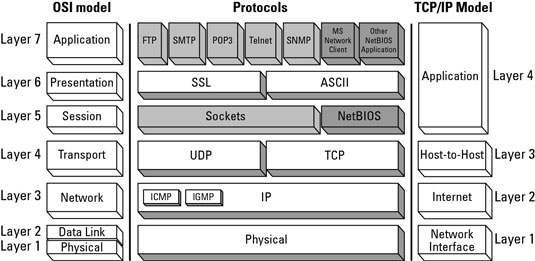
\includegraphics[width=0.7\linewidth]{images/iso_osi_layers.jpg}\\
		\small{\textit{The ISO/OSI model}}
	\end{center}

	\bigbreak
	
	The attack actions categorized by layer are:
	\begin{itemize}
		\item Layer 3: IP, icmp
		\item Layer 4: TCP/UDP
		\item Layer 5 and above: HTTP, DNS, NTP
	\end{itemize}

	\bigbreak
	The defense action is at layer 4. It encrypts the payload of the packets with \lstinline{ChaCha20} algorithm, a \lstinline{Salsa20} modification published in 2008. It is a particularly efficient stream cipher.\\

	\subsection{nfqueue extension}
	NFQUEUE is a kernel and user mode module for managing network packets in iptables. It allows writing \lstinline{Netfilter} target modules in userspace. This module is an application that is called by \lstinline{nfqueue} hooks. In the program, the hooks are bounded to a function that is called when the iptables match a rule.\\
	The function gets the queue details and the packet payload, it can craft the packet, and then send a verdict to the iptables module. 
	
	\bigbreak
	\begin{center}
		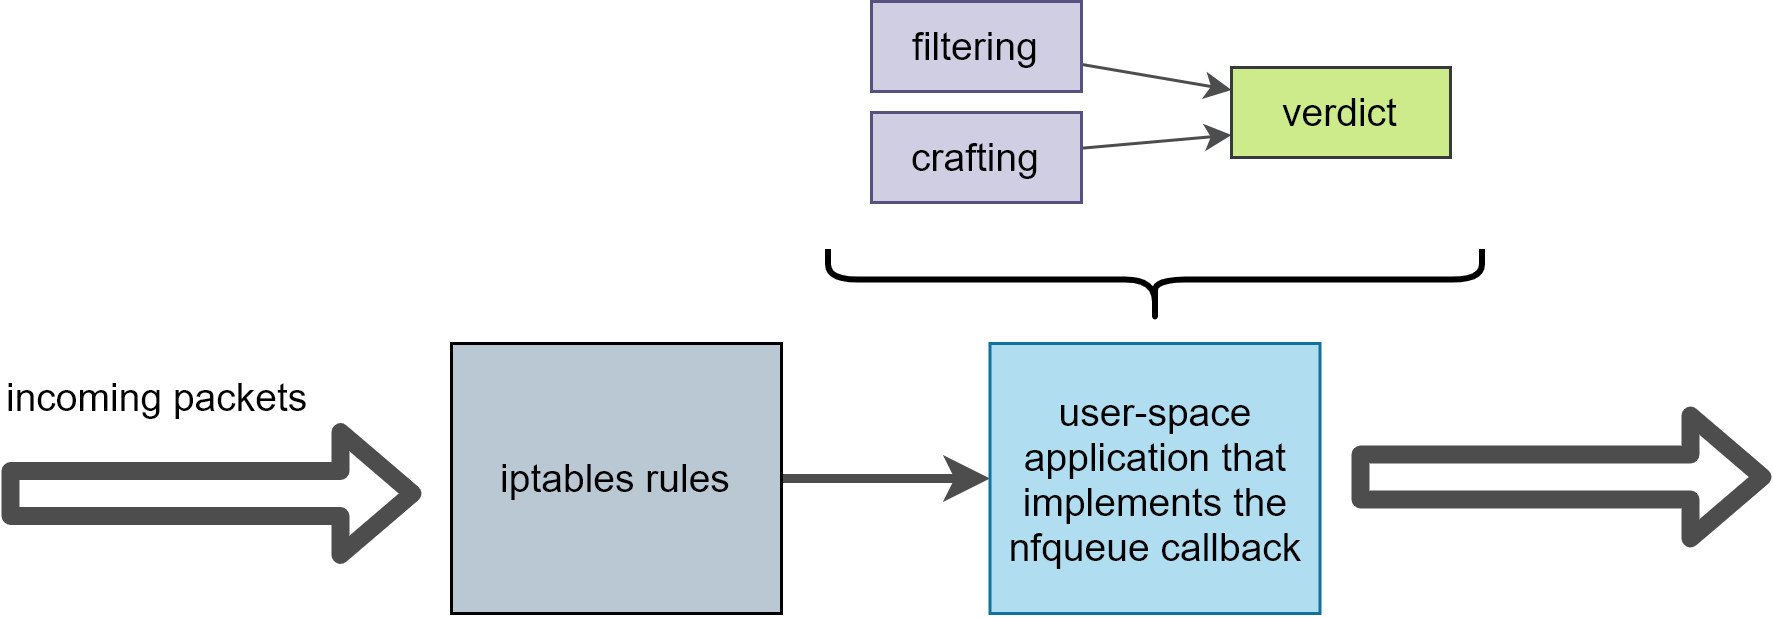
\includegraphics[width=\linewidth]{images/nfqueue_flow.png}\\
		\small{\textit{Flow of the packet}}
	\end{center}
	\bigbreak

	\subsection{PcapPlusPlus}
	It is a multiplatform C++ library for capturing, parsing, and crafting of network packets. As major features, there are that it is designed to be efficient, powerful, and easy to use. It is a wrapper for the most popular packet processing engines making easy decoding and forging a large variety of network protocols.

	\subsection{Software Architecture}
	Craftberry has an architecture composed of four components: the first one is the \lstinline{main} function that sets up the \lstinline{iptables} rules, register the callback function to get the captured packet, and manages the \lstinline{cli} parameters. The second one is the callback function, the core of the application, that takes the captured packets and calls the corresponding action to execute on them. The third component includes all the methods that implement the attack or defense mechanisms. All of them belong to the \lstinline{Action} namespace. The fourth component is a class, called \lstinline{Configuration}, which includes the functions to collect statistics on the elaborated data, and to manage the \lstinline{tun0} network interface. It also implements auxiliary functions for the application.\\

	\subsubsection{The main function}

	We outline the principal sections of the \lstinline{main} function:\\
	The first block of code concerns the registration of the function for external signals, like \lstinline{ctrl+c}. Craftberry can run with a timeout, if the value is passed via CLI, or in infinite mode. In both cases, the execution can be stopped using the external \lstinline{ctrl+c} signal.\\
	\bigbreak

	\begin{lstlisting}[frame=single, language=C++]
		struct sigaction sigIntHandler;
		sigIntHandler.sa_handler = ctrl_c; \\the callback function when the signal is emitted
		sigemptyset(&sigIntHandler.sa_mask);
		sigIntHandler.sa_flags = 0;
		sigaction(SIGINT, &sigIntHandler, NULL);
	\end{lstlisting}
	\bigbreak
	
	The application manages the command-line input parameters using the \lstinline{getopt_long} internal function. The parameters are specified in the \lstinline{help} function output. The input parameters are validated and used to initialize the \lstinline{Configuration} class.\\
	\bigbreak

	The next step is to register the callback function to the \lstinline{nfqueue} when the \lstinline{iptables} rule is matched. To do so, we need to add the rule to the \lstinline{iptables} list. This operation is done by the \lstinline{makeIptableCmd} function described later in the \lstinline{Configuration} class.\\
	\bigbreak

	The main function ends with the infinite loop that reads a buffer pointed by the handler calculated using the \lstinline{nfqueue} initializing function. When the packet matches the \lstinline{iptables} rule, it is moved into the user space memory. Craftberry continuously reads the memory and, when it is not empty, starts the procedure to parse and elaborate the packet.\\

	If the execution has a timeout, we use a separate thread to terminate Craftberry when the timeout is expired. At that time, it is called a procedure to destroy the \lstinline{nfqueue} queue, print an execution summary, free the resources, and delete the \lstinline{iptables} rules.

	\subsubsection{The callback function}

	The callback function is the core of the application. It has the following signature:
	\bigbreak
	
	\begin{lstlisting}[frame=single, language=C++]
		static int callback(struct nfq_q_handle *qh, struct nfgenmsg *nfmsg, struct nfq_data *nfa, void *data);
	\end{lstlisting}
	\bigbreak

	\begin{itemize}
		\item \lstinline{qh}: pointer to the \lstinline{nfqueue} internal handle for the queue;
		\item \lstinline{nfmsg}: pointer to the Netfilter address family dependent message;
		\item \lstinline{nfa}: pointer to the Netfilter captured packet data;
		\item \lstinline{data}: pointer to a user-defined memory to pass context values;
	\end{itemize}
	\bigbreak

	The most important parameter, for our purposes, is \lstinline{nfa} from which we extract the message packet header and payload.\\
	\bigbreak

	\begin{lstlisting}[frame=single, language=C++]
		struct nfqnl_msg_packet_hdr *ph = nfq_get_msg_packet_hdr(nfa);
		unsigned char *rawData = nullptr;
		int len = nfq_get_payload(nfa, &rawData);
		struct pkt_buff *pkBuff = pktb_alloc(AF_INET, rawData, len, 0x1000);
		CHECK(ph == nullptr, "Issue while packet header");
		CHECK(len < 0, "Can't get payload data");
		struct timeval timestamp;
		nfq_get_timestamp(nfa, &timestamp);
	\end{lstlisting}

	Note: we use the MACRO \lstinline{CHECK} to ensure the return values are valid.\\
	\bigbreak
	The \lstinline{pkBuff} variable contains the packet raw data from where we build the PcapPlusPlus \lstinline{RawPacket}. From the \lstinline{RawPacket}, the library is capable of parsing the packet and building all the layers.\\
	\bigbreak

	\begin{lstlisting}[frame=single, language=C++]
		pcpp::RawPacket *inPacketRaw = new pcpp::RawPacket(pktb_data(pkBuff), pktb_len(pkBuff), timestamp, false, pcpp::LINKTYPE_RAW);
		pcpp::Packet *inPacket = new pcpp::Packet(inPacketRaw);
		//Print all packet layers for inspection
		pcpp::Layer *L = p->getFirstLayer();
		while (L != nullptr) {
			cout << "\t\t| LEV: " << L->getOsiModelLayer() << " => " << L->toString() << endl;
			L = L->getNextLayer();
		}
	\end{lstlisting}
	\bigbreak

	The parsed packet is the input for the single operation that the Craftberry user wants to perform.\\
	Each operation is selected matching the action, specified in the passed parameter, and the protocol, recognized in the packet.\\
	\bigbreak
	The pattern is: 
	\bigbreak

	\begin{lstlisting}[frame=single, language=C++]
		if (conf->method.compare("HTTPBLOCK") == 0 && Action::HTTP::isProtocol(inPacket)) {
			//do something with the packet
			return verdict_accept(qh, ntohl(ph->packet_id), inPacket);
		}
	\end{lstlisting}
	\bigbreak

	where, in this example, the passed action is \lstinline{HTTPBLOCK} and \lstinline{inPacket} must contain a HTTP layer.\\
	Every method must end with a call to a \lstinline{verdict} function that decrees if the packet is accepted or dropped.\\
	For the majority of our action implementations, the verdict is to accept the packet that has been modified. Before calling the function to accept the verdict, we collect statistic data and save the packet into a log file. The log file contains all the packets that Craftberry has captured, in case crafted, and accepted to continue the network stack traversal.

	\subsubsection{The action classes}

	The action classes contain the implementation of the attack or defense mechanisms. As said, they belong to the \lstinline{Action} namespace and have a similar common structure. All of them share the \lstinline{isProtocol} method used to identify if the action can be performed on the packet.\\
	The single method that executes the attack or defense mechanism takes in input a \lstinline{Packet} variable, thus a parsed packet. The advantage of using the PcapPlusPlus library is that it exposes functions to craft the packet easily.\\
	\bigbreak
	We describe all the action methods and the relative attack or defense idea in the Action chapter.

	\subsubsection{The Configuration class}
	
	It is a class that follows the \lstinline{singleton} pattern. It contains all the application setup, collects data, and exposes functions used by all the other application components, thus, it is a shared instance.\\
	\bigbreak
	An important function is to open and manage the \lstinline{tun0} network interface using the PcapPlusPlus device management methods. Then it implements the \lstinline{sendPkt} function to send a packet to the destination, the \lstinline{tun0} interface: for some actions this function is needed to complete the attack.\\
	
	\bigbreak

	\begin{lstlisting}[frame=single, language=C++]
		bool sendPkt(RawPacket *p) {
			if (p->getRawDataLen() > conf->devTun0->getMtu()) {
				conf->dropped.packets++;
				conf->dropped.bytes += p->getRawDataLen();
				return false;
			}
			if (conf->devTun0->sendPacket(*p)) {
				conf->created.packets++;
				conf->created.bytes += p->getRawDataLen();
				conf->devLogFile->writePacket(*p);
				return true;
			}
			cout << "something strange just happened" << endl;
			return false;
		};
	\end{lstlisting}
	\bigbreak
	The function also collects data for the statistics.
	\bigbreak

	The \lstinline{Configuration} class also contains the \lstinline{makeIptableCmd} function to add or remove the rule to the \lstinline{iptables} list. It composes the bash command string and then calls the \lstinline{system()} function to execute the command. The function builds the string depending on the actions passed by the function caller and the direction of the packets to capture.\\
	
	\bigbreak

	\begin{lstlisting}[frame=single]
		void makeIptableCmd(bool isDeleting) {
			string protocol = "";
			if (conf->method.compare("BEQUITE") == 0) {
				protocol = "all";
			} else if (conf->method.compare("TCPMULTIPLY") == 0 || conf->method.compare("IPV4") == 0) {
				protocol = "tcp";
			} else ...
			string dir = std::to_string(static_cast<std::underlying_type<Direction>::type>(conf->direction));
			string cmd = ("sudo iptables -t filter "s +
						(!isDeleting ? "-I "s : "-D "s) +
						(conf->direction == 0 ? "INPUT "s : "OUTPUT "s) +
						"-p "s + protocol + " -j NFQUEUE "s +
						" --queue-num "s + dir);
			cout << "IPTABLE RULE: " << endl
				<< "\t$: " << cmd << endl;
			system(("\n#/bin/bash\n\n"s + cmd).c_str());
		};
	\end{lstlisting}
	\bigbreak

	In a scenario where Craftberry is executed two times, once capturing the incoming traffic and once capturing the outgoing traffic, we use the \lstinline{--queue-num nfqueue} parameter to bind the queue with the Craftberry execution. Therefore, the queue number is defined by the packet capturing direction.

	\subsection{Actions}

	\subsubsection{IP}
	The IP packet contains information on the source and the destination IP address. The goal of this attack is to change the destination address to redirect the packet somewhere else.\\
	When the packet is captured from the callback, the \lstinline{changeDst} function is called passing the parsed packet. Then, we extract the IPv4 layer from the stack and change the destination Ip using the PcapPlusPlus methods.\\
	The code is the following:
	\bigbreak

	\begin{lstlisting}[frame=single]
		void changeDst(Packet *inPacket) {
			IPv4Layer *ipv4 = inPacket->getLayerOfType<pcpp::IPv4Layer>();
			ipv4->setDstIpAddress(IPv4Address(newIp));
		}
	\end{lstlisting}
	\bigbreak

	Where \lstinline{newIp} is a class field that contains the new destination IP the attack aims to set. It is set during the action creation.

	\bigbreak
	The scenarios that can use this action are where the attacker wants to redirect all the traffic to another server, often called Command and Control, to perform other activities on the data.   
	
	\subsubsection{ICMP}
	ICMP, an abbreviation for Internet Control Message Protocol, is a protocol used for network messages and diagnostic operations. The action on this level has been implemented for test purposes and does not have any particular attack model. By the way, after capturing the ICMP packet, we are able to change its values for the request and the reply messages.

	\subsubsection{TCP/UDP}
	
	The context of the attack supposes that communication has supplementary encryption, over the VPN encrypted layer, provided by end-to-end encryption between the Mysterium client and the resource server the user is communicating with, and not the exit node. Therefore, the latter cannot perform any content understanding, and can do only actions on the entire packet, as described in the Design vulnerabilities chapter.\\
	The attack accomplishes a simple copy of the packet: when the provider receives packets from the internet, it sends \lstinline{n} times a copy of the captured packet to the consumer.\\
	The implementation is as simple as significant: with this method, with no content understanding, the passing data are more than the necessary, and the service consumer is affected.\\
	\bigbreak
	We have implemented a demonstrative example of this attack using the protocols TCP and UDP.\\
	\bigbreak
	The code in the main function is the following:\\
	\begin{lstlisting}[frame=single]
		if (conf->method.compare("ICMPMULTIPLY") == 0 && Action::Icmp::isProto(inPacket)) {
			Action::Tcp *action = new Action::Tcp(n);
			action->multiply(inPacket->getRawPacket());
			return verdict_accept(qh, ntohl(ph->packet_id), inPacket);
		}
	\end{lstlisting}

	\bigbreak
	The multiply method is implemented as follows:
	\bigbreak
	\begin{lstlisting}[frame=single]
		void multiply(RawPacket *inPacket) {
			for (int i = 0; i < this->n; i++) {
				sendPkt(inPacket);
			}
		}
	\end{lstlisting}
	\bigbreak

	The \lstinline{n} parameter is a TCP class field.\\
	For each received TCP packet, the method send \lstinline{n} copies of it to the network.

	\subsubsection{DNS robber}

	The DNS is a network protocol necessary to resolve a domain name to the correspondent address. Unfortunately, it is unencrypted and susceptible to attacks of a different nature \cite{DNSATTACKS}.\\
	The attack idea is to capture a DNS request and response and perform DNS hijacking \cite{DNShijacking}. The hijacking can be done in different ways: capturing the DNS request or capturing the DNS response.\\
	\bigbreak	
	The request contains the name server the machine wants to resolve to get the corresponding IP address necessary to begin the communication. If we catch the request packet, we can change the name server with another malicious nameserver under our control. The DNS resolver reply to the consumer with our machine IP that returns our web page, if the query is HTTP. This attack can be used for phishing, the attempts to obtain sensitive information by disguising oneself as a trustworthy entity, or for collecting data.\\
	The response packet modification has a similar goal, and the attack has the same impact: to block a specific name server or to force all the requests to a different IP address. The latter scenario can be the central action to perform a denial of service, overloading a server of, in our example, HTTP requests.
	
	\subsubsection{HTTP}

	Hypertext Transfer Protocol is an application-layer protocol for transmitting hypermedia documents, and it is the standard in the client-server architectures. The HTTP protocol is stateless, meaning that the server does not keep any state between two requests.\\
	This protocol is perfect for implementing an attack and for demonstrating how a node can maliciously and heavily modify the content of a packet. Our goal is to intercept the response of the HTTP answer, detect if the payload is an image, and then substitute it with another one. We need to clarify that the HTTP response content can be split over many TCP packets, if it is larger than the maximum TCP packet size. Craftberry captures TCP packets but does not perform TCP reassembly. Therefore, for our demonstration purpose, it can operate the image substitution only for images contained in a single TCP frame.\\
	
	\bigbreak
	A little variant of this attack changes the URL of the \lstinline{GET} method of the HTTP request.\\
	For example, if the HTTP request is in the form:\\
	
	\bigbreak
	\begin{lstlisting}[frame=single]
		URL: http://www.example.com/resource
	\end{lstlisting}
	\bigbreak
	
	it becomes
	
	\bigbreak
	\begin{lstlisting}[frame=single]
		URL: http://www.maliciouswebsite.com?p=http://www.example.com/resource
	\end{lstlisting}
	\bigbreak
	
	When the malicious website gets the request, it collects data and redirects to the original website.\\
	The ultimate goal is to perform aggressive advertisement campaigns.\\
	\bigbreak

	As further action implementation, we made a web filter. The method checks the HTTP request and drops the packets that match the blocked URL. The action in the Craftberry application is called \lstinline{HTTPBLOCK}.

	\subsubsection{Cipher}

	This action is a conceptual proposal of a defense mechanism to protect the traffic. The idea is to use a fast and efficient cipher algorithm, such as Salsa20, to encrypt all the outgoing content and decrypt all the incoming content. The encryption operation is performed on the TCP payload. It expects to dialog with another cipher/decipher entity positioned on the service provider point or on another server that can be reached outside the VPN tunnel.\\
	\bigbreak

	\subsection{Tests}
		Following, we show a complete example of execution.\\
		The input specifies the action to block the outgoing HTTP requests.
		\bigbreak
		\begin{lstlisting}[frame=single]
		make all && sudo ./craftberry -I 10.135.63.160 -a HTTPBLOCK -d OUT
		\end{lstlisting}
		\bigbreak
		The following is the working output of Craftberry that prints a setup summary and then the captured packets.
		\bigbreak
		\begin{lstlisting}[frame=single]
		Method:                HTTP
			Logfile:               captures/out_1584126885.pcapng
			Direction:             OUT
		Interface tun0 info:
			IP:                    10.135.63.160
			Interface name:        eth1
			Interface description: 
			MAC address:           62:26:9f:43:ed:c3
			Default gateway:       0.0.0.0
			Interface MTU:         1500
			DNS Servers:           0
		IPTABLE RULE: 
			$: sudo iptables -t filter -I OUTPUT -p tcp -m multiport --dports 80,443 -j NFQUEUE  --queue-num 1
		Working in infinity mode, press ctrl+c to exit...
		| LEV: 3 => IPv4 Layer, Src: 165.22.66.6, Dst: 82.196.9.250
		| LEV: 4 => TCP Layer, [ACK], Src port: 33167, Dst port: 443
		| LEV: 6 => TLSv1.2 Layer, Application Data

		| LEV: 3 => IPv4 Layer, Src: 165.22.66.6, Dst: 82.196.9.250
		| LEV: 4 => TCP Layer, [FIN, ACK], Src port: 33167, Dst port: 443

		| LEV: 3 => IPv4 Layer, Src: 165.22.66.6, Dst: 82.196.9.250
		| LEV: 4 => TCP Layer, Src port: 33167, Dst port: 443
		.....
		\end{lstlisting}

		\bigbreak
		Finally, when the application finishes, it prints a performance summary.
		\begin{lstlisting}[frame=single]
		^C
		Ooooops got ctrl+c signal (2)
		Here a summary of what happened:
		Packets received:      147 (11760 bytes)
		Packets crafted:       0 (0 bytes)
		Packets created:       0 (0 bytes)
		Packets dropped:       147 (11760 bytes)
		All is clean
		IPTABLE RULE: 
				$: sudo iptables -t filter -D OUTPUT -p tcp -m multiport --dports 80,443 -j NFQUEUE  --queue-num 1
		bye bye
		\end{lstlisting}
		\bigbreak
		We performed several tests on the Craftberry application that regarded the different actions and the different contexts where the app can work. Even if the app is a prototype, we successfully demonstrated its main purpose: to shows the Mysterium Network vulnerability for what concerns the exit nodes.\\
		The tests also focused on the performance impacts: our results show the overhead is minimum thanks to the use of efficient technologies, the C++ language and the PcapPlusPlus library in particular.
		

	\subsection{Design solutions for malicious context}

		The Mysterium Network is, as previously described, vulnerable in several scenarios. The exit nodes control the incoming and outgoing data and can perform different actions on it. Furthermore, the introduction of the multihop topology does not seem to avoid this problem.\\
		\bigbreak
		In this section, we analyze the possible solutions from the consumer perspective. They do not solve all the problems but try to increase the reliability of the network.\\

		\subsubsection{Decoy data}
		The decoy data are known resources the client already has.
		In this first solution that we analyze, the client requests these decoy data at a variable frequency to check the data integrity. The ultimate goal is to compare the data obtained from the VPN connection with the data the client has. If the resources match it means the exit node did not alter the traffic content.\\
		\bigbreak
		This method does not provide the certainty that all the traffic has not been modified. More we increase the frequency of the decoy data requests, and more the integrity reliability increases. On the other hand, the connection cost grows up linearly with the frequency of the request.\\
		Another supposition regards the exit node capability to adapt itself to this scenario. It can easily detect a frequent request to the same resource and deduct that the client is using decoy data to perform a connection integrity check.\\To solve this problem, the client should increase the number of known resources so that every request is addressed to a different decoy data.\\
		These considerations make the method unfeasible to implement.

		\subsubsection{Duplicated data}
		A different approach to the previous method consists of requesting the same resource to two different nodes and then compare the two obtained data. This method needs the client node connected to two nodes at the same time. This is not possible with the current Mysterium Network implementation. Furthermore, it is costly because it doubles the connection cost.\\
		Another limitation regards the nature of the resource: if it is stateful, the double request breaks the consistency of the states.
		 
		\subsubsection{Data hashes}
		A little variant of the duplicated data approach consists of changing the duplicated content: from the whole data to its hash.\\
		The hash function is a mathematical algorithm that maps data of arbitrary size to a bit string of a fixed size. It is a one-way function commonly used in cryptography. We can consider the hash of a file like its fingerprint. In our solution, the client has a main connection from where it gets the resource and other connections that provide the hashes of the same resources. When the client gets the resource, it calculates its hash and compares it with the hashes obtained from the other connections. The hashes must match to determinate the exit node of the main connection did not alter the returned data. Also, the hash function must be the same between all the nodes, consumers and providers.\\
		\bigbreak
		This solution does not fit with stateful connections as well, but cut the costs for the client.\\
		\bigbreak
		We implement a prototype of this last solution.\\
		Currently, Mysterium Network does not support connection to many exit nodes at the same time; only one VPN tunnel is supported. Therefore, we used Docker to run two instances of the Mysterium client mapped on two different ports. Then, using a bash script, we requested the same resource and, once obtained the data, we performed the comparison.\\
		To simulate the hash function on the exit nodes, we implemented a specific action on Craftberry that transforms the content of a specific resource request to its hash value. We used the \lstinline{MD5} function for simplicity. We do not use \lstinline{MD5} for security application since it has been declared broken \cite{MD5hash}, but only to get a fast fingerprint of the file.\\
	
		\bigbreak
		\begin{center}
			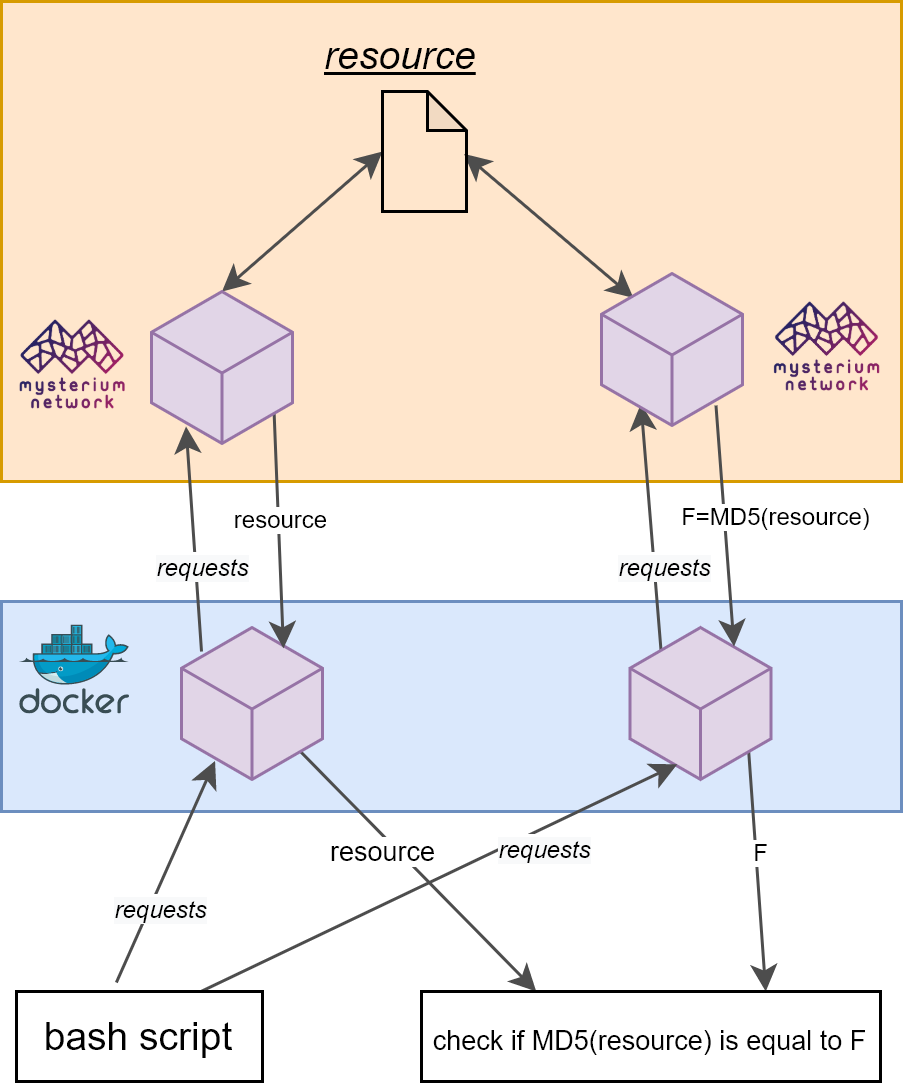
\includegraphics[width=0.7\linewidth]{images/comparing_data_architecture.png}\\
			\small{\textit{Hashes data comparison}}
		\end{center}
		\bigbreak
		
		As described, if the two \lstinline{md5} hashes match, it means the exit node of the main connection did not modify the returned content, yes otherwise.

	\newpage
	\section{Conclusions}
		\subsection{Future development}
			There are two future development paths the Craftberry application can take: the first one regards the implementation of other attack or defense mechanisms to extend the possible scenario where Craftberry can act. The second one, for us the most interesting, regards the enhancement of specific attacks. For instance, the TCP/UDP packet multiplication could be refined and improved to exploit the end node critical role fully.\\
			If the Craftberry application becomes popular in the Mysterium Network community, many other scenarios could take place: for instance, a coordinated attack of all nodes against a specific server or network can lead to distributed denial of service, acting as a botnet.\\
			\bigbreak
			Another branch of future development regards the reputation systems that a network, like Mysterium Network, could integrate to improve the users' management inside the network.

			\subsection{Considerations}
			At the end of this research, we can say that the Mysterium Network is a promising solution to keep safe our online identities and protect our browsing. Nevertheless, the vulnerabilities we analyzed make the product not mature enough to be used commercially, in our opinion.\\
			The level of security we currently have to protect us browsing or for online activities is not sufficient. Projects like Mysterium Network are necessary to enhance it. Our motivations behind the study of Mysterium Network are to expose its weakness so they can be patched for a final improvement of the project. For this reason, Craftberry wants to be a demonstrative tool, and we do not suggest or encourage its use for any usage apart from the research one.
			
			\bigbreak

			For what concerns our demonstrative tool, a significant milestone has been reached: the technical solution to use Netfilter Queue Library to capture the inline packets and PcapPlusPlus to parse them. The Craftberry application represents a working example of how the two technologies can work together.\\
			Furthermore, Craftberry is the first tool that interacts with the Mysterium Network project in the community, and we hope it can be the starting point for other projects.  

			\bigbreak

			This research is the result of a long work on the Mysterium Network project. It has changed several times from its born until now, forcing us to adapt to it. Therefore, we can not assure the conclusions we reached here will be valid in the future. For some of them, we hope they will not, meaning the project improved its design.\\
			In conclusion, we reached most of the goals defined at the beginning of the work. The reputation systems analysis we wanted to include in this research has not been covered because it would have changed the focus of the study.

	\pagebreak

	{\bfseries\Large Thanks}\\
	to me, myself, and whom I see in the morning when I look at the mirror.

	\pagebreak

	\bibliographystyle{plain}
	\begin{thebibliography}{1}
		\bibitem{UnsecureVpns}
			The risks of vpns\\
			\url{https://www.trendmicro.com/vinfo/us/security/news/cybercrime-and-digital-threats/shining-a-light-on-the-risks-of-holavpn-and-luminati}
		\bibitem{MD5hash}
			The MD5 hash is broken\\
			\url{https://www.schneier.com/blog/archives/2008/12/forging_ssl_cer.html}
		\bibitem{HTTPS}
			HTTP Over TLS - RFC\\
			\url{https://tools.ietf.org/html/rfc2818}
		\bibitem{VPNRFC}
			A Framework for IP Based Virtual Private Networks - RFC\\
			\url{https://tools.ietf.org/html/rfc2764}
		\bibitem{tc}
			Traffic Control\\
			\url{https://jvns.ca/blog/2017/04/01/slow-down-your-internet-with-tc/}
		\bibitem{tc}
			An Analysis of the Privacy and Security Risks of
Android VPN Permission-enabled Apps\\
			\url{https://research.csiro.au/ng/wp-content/uploads/sites/106/2016/08/paper-1.pdf}
		\bibitem{exitnodeTOR}
			Tor Network - Exit nodes\\
			\url{https://www.wired.com/2007/09/rogue-nodes-turn-tor-anonymizer-into-eavesdroppers-paradise/?currentPage=all}
		\bibitem{exitnodeTOR2}
			TOR Network - Malicious exit nodes\\
			\url{https://www.makeuseof.com/tag/priority-wretched-hive-scum-villainy-5-ways-stay-safe-bad-tor-exit-nodes/}
		\bibitem{exitnodeTOR3}
			TOR - trust exit nodes\\
			\url{https://nakedsecurity.sophos.com/2015/06/25/can-you-trust-tors-exit-nodes/}
		\bibitem{DeanonymizingTorCircuits}
			Deanonymizing Tor Circuits\\
			\url{https://www.hackerfactor.com/blog/index.php?/archives/868-Deanonymizing-Tor-Circuits.html}
		\bibitem{DNSATTACKS}
			DNS attack patterns\\
			\url{https://www.fireeye.com/blog/threat-research/2019/01/global-dns-hijacking-campaign-dns-record-manipulation-at-scale.html}
		\bibitem{DNSATTACKS2}
			DNS leaks\\
			\url{https://securitytrails.com/blog/what-is-dns-leak-how-can-i-prevent-it}
		\bibitem{DNShijacking}
			DNS hijacking\\
			\url{https://securitytrails.com/blog/dns-hijacking}
		\bibitem{NetfilterLibrary}
			Netfilter Queue Extension Library\\
			\url{https://home.regit.org/netfilter-en/using-nfqueue-and-libnetfilter_queue/}
		\bibitem{TUNTAP}
			TUN/TAP\\
			\url{https://buffered.com/glossary/tun-tap/}
		\bibitem{TCPDUMP_linktypes}
			Tcpdump link types\\
			\url{https://www.tcpdump.org/linktypes.html}
		\bibitem{NFQueue_PcapPlusPlus Integration}
			Netfilter queue extension and PcapPlusPlus integration\\
			\url{https://netfilter.org/projects/libnetfilter_queue/doxygen/html/group__nfq__verd.html}
		\bibitem{PcapPlusPlusNetfilter}
			Netfilter queue extension and PcapPlusPlus integration\\
			\url{https://groups.google.com/forum/#!msg/pcapplusplus-support/e7rN93LfTSg/MFnVEKCNCAAJ}
		\bibitem{NetfilterMITM}
			Netfilter queue MITM attack\\
			\url{https://www.apriorit.com/dev-blog/598-linux-mitm-nfqueue}
		\bibitem{NetfilterPython}
			Netfilter queue with python\\
			\url{https://byt3bl33d3r.github.io/using-nfqueue-with-python-the-right-way.html}
		\bibitem{NetfilterQueueSnapy}
			Netfilter queue with Snapy	\\		
			\url{https://stackoverflow.com/questions/27293924/change-tcp-payload-with-nfqueue-scapy}
		\bibitem{VPNsellData}
			VPN seel data to third parties\\
			\url{https://thenextweb.com/contributors/2018/05/28/be-cautious-free-vpns-are-selling-your-data-to-3rd-parties/}
		\bibitem{OpenVPNInternalSchema}
			OpenVPN Internal Schema\\
			\url{https://subscription.packtpub.com/book/networking_and_servers/9781783553136/1/ch01lvl1sec12/openvpn-internals}
		\bibitem{MysteriumWhitePaper}
			Mysterium White Paper\\
			\url{https://mysterium.network/whitepaper.pdf}
		\bibitem{PcapPlusPlusLibrary}
			PcapPlusPlus Library\\
			\url{https://pcapplusplus.github.io/docs/features}

	\end{thebibliography}
		
	\pagebreak
	
	%%	{\Large Valutazione di un nuovo utente della rete}
	\paragraph{Contesto}
	Rete VPN decentralizzata attiva e con connessione multi-hop tra una generica coppia Agent-Client.
	
	\paragraph{Problema 1: identificare gli Agent in posizione endnode che inviano contenuto non originale}
	In una rete VPN decentralizzata gli Agent endnode hanno il compito di recuperare una risorsa web e restituirla al Client attraverso la rete VPN instaurata. L'Agent, che quindi ha accesso intrinseco al dato ottenuto, cifrato o meno, può modificarlo prima di inviarlo al Client. Questa operazione può avere scopi malevoli, tra cui quello del guadagno economico. In possibile scenario, in questo contesto, è quello che vede l'incremento della grandezza del pacchetto da Agent a Client al fine di maggiorare i consumi della banda stabilita nel contratto iniziale di fornitura del servizio.
	
	\paragraph{Problema 2: scoraggiare abusi della rete}
	Per scoraggiare abusi della rete si utilizza una \textit{prova di lavoro} (Proof of Work) per attestare che il nuovo utente della rete ha speso delle risorse al fine di guadagnare reputazione nel contesto distruibuito.\\
	La reputazione iniziale, all'ingresso della rete distribuita, ha valore zero.
	
	\paragraph{Soluzione problema 1}
	\begin{itemize}
		\item Dati civetta: è richiesta dal Client all'Agent, con frequenza variabile, una risorsa dal valore noto al Client per la verifica di integrità. Se il test risulta negativo si ipotizza la modifica della risorsa da parte dell'Agent.
		\item Dati duplicati: il Client si connette a due Agent diversi e chiede ad entrambi la risorsa desiderata, alla ricezione si comparano per la verifica di integrità. Se il test risulta negativo si ipotizza la modifica della risorsa da parte di uno dei due Agent.\\
		\textbf{Aspetti negativi:} questa soluzione non è applicabile in caso di connessioni con la risorsa che prevedono \textit{stati}.(??)
		\item Hash Dato: il Client si connette ad un Agent al quale chiede una risorsa e successivamente chiede ad un altro Agent l'hash della risorsa stessa. Il Client effettua quindi un hash (stessa funzione hash) della risorsa ottenuta dall'Agent e la compara con l'hash ottenuto dal secondo Agent. Ulteriore implementazione può essere effettuata richiedendo a più agent l'hash della risorsa.\\
		Se il test risulta negativo si ipotizza la modifica della risorsa da parte del primo Agent.\\
		\textbf{Aspetti negativi:} questa soluzione non è applicabile in caso di connessioni con la risorsa che prevedono \textit{stati}.\\
		\textbf{Caso d'uso:} si reputa questo metodo adatto a verificare un Agent al suo primo ingresso nella rete in quanto non è spesso adatto per l'aspetto negativo sopra descritto.		
	\end{itemize}
	
	\paragraph{Soluzione problema 2}
	L'originalità della soluzione proposta è l'operazione di Proof of Work da far compiere al nuovo utente. Si propone come prova di lavoro che l'utente, prima di entrare attivamente a far parte della rete o durante la sua partecipazione, consumi della banda internet.\\
	La Proof of Work, quindi, consiste nello sfruttare la sua banda internet per ottenere una risorsa internet, sulla quale viene verificata l'integrità, come descritto nella soluzione \textit{Dato Hash} proposta nella soluzione al problema 1.\\ 
	Più specificatamente, nel caso d'uso si identificano un Agent A, un Client C ed un nuovo utente X che vuole entrare nella rete e deve dimostrare \textit{la prova di lavoro}.\\
	La situazione iniziale prevede una connessione tra A e C. Per verificare che A fornisca dato $d^A$ originale, C richiede a X di ottenere lo stesso dato $d^X$ e di eseguirne la funzione hash così da ottenere  $H(d^X)=h_1$. $h_1$ sarà restituito a C che ha già effettuato la stessa funzione hash su $d^A$ proveniente da A ed ha ottenuto $H(d^A) = h_2$.\\
	Il test di integrità verifica che $h_1 = h_2$.\\
	Se il test ha successo si ha certezza che:
	\begin{enumerate}
		\item il nuovo utente X ha eseguito correttamente la proof of work 
		\item A ha fornito a C un dato originale, a meno che sia A che X applichino le stesse modifiche al dato prima di effettuarne la funzione hash.\\Questa vincolo è da verificare.
	\end{enumerate}
	
	\paragraph{Considerazioni}
	In un contesto di rete distribuita si possono ipotizzare $n$ attori nel ruolo di X e $n$ test di integrità che C effettua per verificare l'integrità del dato ottenuto da A. \textit{riferimento al consenso BFT}\\
	Il risultato dei test condiziona la reputazione di ogni attore nel ruolo di $X$.\\
	Si può ipotizzare l'applicazione della soluzione $m$ volte, tante quante sono le entità per cui effettuare la proof of work, e considere vincoli come tempo $t$ minimo di esecuzione della proof of work o la quantità minima di dati $q$ che $X$ deve ottenere su cui applicare la funzione hash.\\
	
	
	Considerando una costo ipotetico $c$ associato al consumo di una quantità $q$ di dati per un'unità di tempo $t$ si può impostare una soglia $S = c*q*t$ superata la quale la proof of work si può considerare eseguita.\\
	L'ultima affermazione garantisce l'asimmetria della proof of work (??). (che è: hash difficile da calcolare perchè spendo risorsa di tempo e di banda e facile da verificare dal client perchè effettuo un semplice confronto di un hash)(vedere https://it.wikipedia.org/wiki/Hashcash per similitudini sulla variabile del tempo)\\
	
	
	La reputazione di ogni entità all'interno della rete, sia Agent che Client, subisce una variazione in quanto ciascun esito delle proof of work viene registrata nella blockchain e questo consente di avere una classifica di affidabilità delle entità quasi in tempo reale.\\
	

	

\end{document}